\documentclass[11pt]{article}

% Change "review" to "final" to generate the final (sometimes called camera-ready) version.
% Change to "preprint" to generate a non-anonymous version with page numbers.
\usepackage{acl}

% Standard package includes
\usepackage{times}
\usepackage{latexsym}

% For proper rendering and hyphenation of words containing Latin characters (including in bib files)
\usepackage[T1]{fontenc}
% For Vietnamese characters
% \usepackage[T5]{fontenc}
% See https://www.latex-project.org/help/documentation/encguide.pdf for other character sets

% This assumes your files are encoded as UTF8
\usepackage[utf8]{inputenc}

% This is not strictly necessary, and may be commented out,
% but it will improve the layout of the manuscript,
% and will typically save some space.
\usepackage{microtype}

% This is also not strictly necessary, and may be commented out.
% However, it will improve the aesthetics of text in
% the typewriter font.
\usepackage{inconsolata}

%Including images in your LaTeX document requires adding
%additional package(s)
\usepackage{graphicx}

\usepackage{booktabs}
\usepackage{multirow}
\usepackage{amsmath}
\usepackage{tcolorbox}
\usepackage{listings}
\usepackage{blindtext}
\usepackage{cleveref}

% If the title and author information does not fit in the area allocated, uncomment the following
%
%\setlength\titlebox{<dim>}
%
% and set <dim> to something 5cm or larger.

\title{Comprehensive Comparison of RAG Methods Across \\Multi-Domain Conversational QA}

% Author information can be set in various styles:
% For several authors from the same institution:
% \author{Author 1 \and ... \and Author n \\
%         Address line \\ ... \\ Address line}
% if the names do not fit well on one line use
%         Author 1 \\ {\bf Author 2} \\ ... \\ {\bf Author n} \\
% For authors from different institutions:
% \author{Author 1 \\ Address line \\  ... \\ Address line
%         \And  ... \And
%         Author n \\ Address line \\ ... \\ Address line}
% To start a separate ``row'' of authors use \AND, as in
% \author{Author 1 \\ Address line \\  ... \\ Address line
%         \AND
%         Author 2 \\ Address line \\ ... \\ Address line \And
%         Author 3 \\ Address line \\ ... \\ Address line}

\author{
 \textbf{Klejda Alushi},
 \textbf{Jan Strich},
 \textbf{Chris Biemann,
 \textbf{Martin Semmann}
 }\\
 Hub of Computing and Data Science (HCDS) \\
 University of Hamburg, Germany \\
 \\
 \small{
   \textbf{Correspondence: \texttt{\{first\_name\}.\{last\_name\}@uni-hamburg.de}}
 }
}
%\author{
%  \textbf{First Author\textsuperscript{1}},
%  \textbf{Second Author\textsuperscript{1,2}},
%  \textbf{Third T. Author\textsuperscript{1}},
%  \textbf{Fourth Author\textsuperscript{1}},
%\\
%  \textbf{Fifth Author\textsuperscript{1,2}},
%  \textbf{Sixth Author\textsuperscript{1}},
%  \textbf{Seventh Author\textsuperscript{1}},
%  \textbf{Eighth Author \textsuperscript{1,2,3,4}},
%\\
%  \textbf{Ninth Author\textsuperscript{1}},
%  \textbf{Tenth Author\textsuperscript{1}},
%  \textbf{Eleventh E. Author\textsuperscript{1,2,3,4,5}},
%  \textbf{Twelfth Author\textsuperscript{1}},
%\\
%  \textbf{Thirteenth Author\textsuperscript{3}},
%  \textbf{Fourteenth F. Author\textsuperscript{2,4}},
%  \textbf{Fifteenth Author\textsuperscript{1}},
%  \textbf{Sixteenth Author\textsuperscript{1}},
%\\
%  \textbf{Seventeenth S. Author\textsuperscript{4,5}},
%  \textbf{Eighteenth Author\textsuperscript{3,4}},
%  \textbf{Nineteenth N. Author\textsuperscript{2,5}},
%  \textbf{Twentieth Author\textsuperscript{1}} 
%\\
%\\
%  \textsuperscript{1}Affiliation 1,
%  \textsuperscript{2}Affiliation 2,
%  \textsuperscript{3}Affiliation 3,
%  \textsuperscript{4}Affiliation 4,
%  \textsuperscript{5}Affiliation 5
%\\
%  \small{
%    \textbf{Correspondence:} \href{mailto:email@domain}{email@domain}
%  }
%}


\begin{document}
\maketitle

\begin{abstract}
Conversational question answering increasingly relies on retrieval-augmented generation (RAG) to ground large language models (LLMs) in external knowledge. Yet, most existing studies evaluate RAG methods in isolation and primarily focus on single-turn settings. This paper addresses the lack of a systematic comparison of RAG methods for multi-turn conversational QA, where dialogue history, coreference, and shifting user intent substantially complicate retrieval. We present a comprehensive empirical study of vanilla and advanced RAG methods across eight diverse conversational QA datasets spanning multiple domains. Using a unified experimental setup, we evaluate retrieval quality and answer generation using generator and retrieval metrics, and analyze how performance evolves across conversation turns. Our results show that robust yet straightforward methods, such as reranking, hybrid BM25, and HyDE, consistently outperform vanilla RAG.
In contrast, several advanced techniques fail to yield gains and can even degrade performance below the No-RAG baseline. We further demonstrate that dataset characteristics and dialogue length strongly influence retrieval effectiveness, explaining why no single RAG strategy dominates across settings. 
Overall, our findings indicate that effective conversational RAG depends less on method complexity than on alignment between the retrieval strategy and the dataset structure.
We publish the code used.\footnote{\href{https://github.com/Klejda-A/exp-rag.git}{GitHub Repository}}

\end{abstract}

\section{Introduction} \label{ch:1-introduction}
Conversational search, the task of satisfying information needs through multi-turn dialogue, has gained significant traction due to recent advances in LLMs~\citep{mo_survey_2025}.
The field is shifting from traditional keyword-based queries to conversational search, characterized by multi-turn natural-language interactions that capture complex and evolving information needs~\citep{mo_survey_2025, prayitno_conversational_2025}. 
To support these interactions, RAG has emerged as the de facto standard~\citep{lewis_retrievalaugmented_2020, huang_survey_2024, nikishina_creating_2025}. By retrieving external evidence from vector databases, RAG mitigates hallucinations and ensures responses are factually grounded and up-to-date~\citep{shuster_retrieval_2021, sahoo_comprehensive_2024}.

\begin{figure}[!t]
\begin{center}
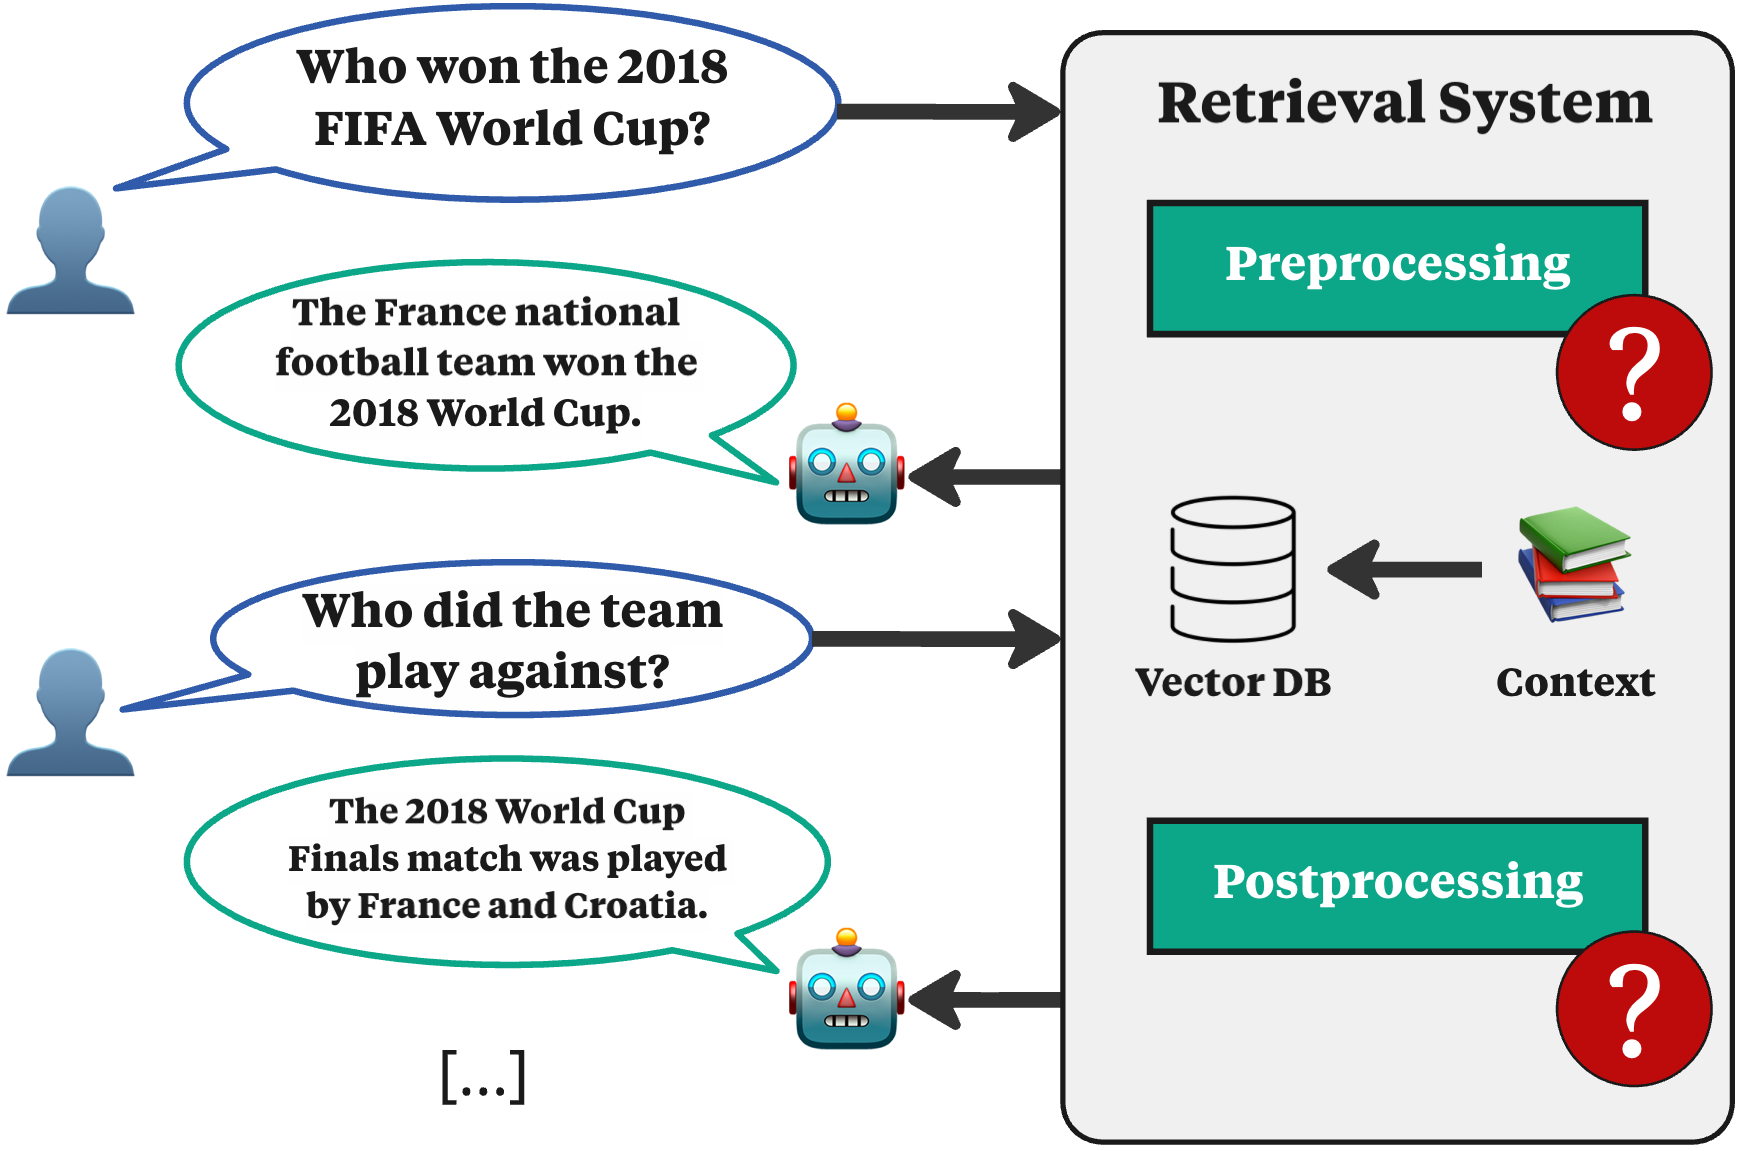
\includegraphics[width=1\columnwidth]{plots/overview4.png}
\caption{Conversational Search Problem. One sample from the INSCIT dataset~\cite{wu_inscit_2023}. }
\label{fig:overview}
\end{center}
\end{figure}



While RAG is well established for single-turn Question Answering (QA), effectively integrating external knowledge into multi-turn conversations introduces significant complexity. In this setting, the system must maintain context across the dialogue history, resolving coreference and handling implicit queries when information is omitted (e.g., ellipsis). Consequently, retrieval effectiveness can vary widely depending on the system's ability to track dialogue history, resolve ambiguity, and adapt to shifting user intent across turns~\citep{saharoy_evidence_2025, chang_mainrag_2025, zhang_dhrag_2025}.
Although the literature reports a rapid evolution of advanced RAG architectures~\citep{gao_retrievalaugmented_2023, huang_survey_2024} and optimization strategies~\citep{gao_complement_2021, gao_precise_2023}, these methods are typically evaluated in isolation~\cite{yu_evaluation_2025}.

Currently, the field lacks a comprehensive overview of RAG strategies for conversational settings. Existing studies often utilize only vanilla RAG~\cite{liu_chatqa_2024, xu_chatqa_2025}, lacking SOTA retrieval metrics, limiting reproducibility, and practical insights for RAG in production systems. 
Furthermore, the interplay between retrieval performance and the depth of the conversation, specifically how performance degrades or changes as the dialogue progresses, remains underexplored.

To address this gap, we present an empirical analysis of RAG methods for conversational QA.
Our contributions are as follows: 
\begin{itemize}
    \item We provide a unified comparison of vanilla RAG and \textbf{six advanced RAG methods} under a reliable evaluation on \textbf{eight conversational QA datasets.}
    \item We further analyze the influence of the \textbf{position of the conversational turn} on retrieval performance. 
\end{itemize}




%This lack of systematic evaluation highlights the need for a rigorous and controlled study of RAG methods in conversational search. Prior work has shown that retrieval quality and grounding substantially affect downstream answer correctness in conversational QA systems \citep{lewis_retrieval-augmented_2020, shuster_retrieval_2021, sahoo_comprehensive_2024}. However, existing studies typically evaluate individual methods in isolation, often under differing datasets and experimental settings, limiting comparability and reproducibility \citep{gao_retrieval-augmented_2023, huang_survey_2024}. Moreover, conversational context introduces additional complexity, as retrieval effectiveness may vary across dialogue turns and information needs \citep{prayitno_conversational_2025, saha_roy_evidence_2025}. These gaps motivate a unified empirical analysis of RAG strategies for conversational search.



%Despite the advancements mentioned above, there are still some issues that have arisen. One of those is that after the LLMs are trained, it becomes much more computationally and financially difficult to retrain them with up-to-date data. This means that for long periods of time, LLMs may be using inaccurate or obsolete data, thus reducing their reliability for factual information and increasing the chance of generating false or contradicting data \cite{DBLP:conf/emnlp/MousaviAR24}. 
%Another problem that has arisen is the narrow range of datasets used in comparative surveys, which can set misleading performance expectations for datasets with differing structures, such as tabular or dialogue-based datasets or datasets. The lack of testing for these datasets can cause various problems ranging from the incorrect processing of input data, to the overstatement of the significance of outliers or minor biases \cite{pal_domain-specific_2024}. Furthermore, generation issues can arise, in which  the generated outcome might not be in the desired format or might include hallucinated information \cite{DBLP:journals/corr/abs-2401-11817}.


%This is where the second method, RAG, comes in, which aims to use external data sources more quickly and efficiently.
%RAG uses various search and retrieval methods to scan an external database, collect the documents that best match the given user query, and use the information within those documents to generate a response \cite{DBLP:conf/kdd/FanDNWLYCL24}.
%This core process of RAG, also known as \textit{Naive RAG}, faces some significant challenges. Retrieval problems such as inadequate text segmentation \cite{zhang2025sage} or unclear input queries may lead to imprecise or noisy retrieved contexts, which can distract LLMs and impede their performance \cite{shi2023large}. 


%This paper aims to tackle these issues by providing a thorough comparison of multiple conversational QA datasets across a variety of advanced RAG methods. This will be accompanied by an analysis of dataset characteristics and the impact that they have on the performance. The performance will likewise be measured across a number of metrics, both to measure the validity of the answer, and the retriever's accuracy and recall. 

%Advanced RAG methods build upon the baseline version by enhancing parts of the RAG pipeline resulting in longer runtimes, the need for extra computational complexity, and a substantial increase in the number of prompts, which when using proprietary models can lead to higher monetary costs. Thus, it will be valuable to investigate whether the potential increased performance of advanced RAG methods justify these drawbacks. 




%These problems have led to the development of many advanced RAG algorithms, which employ many pre- and post-retrieval enhancements, and modular RAG algorithms, which combine these enhancements, all the while transcending the traditional linear structure using loops, conditions, and branching \cite{gao2024modular}. This paper looks into these different techniques to determine whether they lead to an improvement in performance, and if so, to what extent and in which manner.




%The advanced RAG methods that will be looked at all add extra layers of complexity to the baseline RAG method, which can result in the need for more processing power, insufficient time constraints, and an increase in LLM prompts, which, when using proprietary models, lead to higher monetary costs. Therefore, to make some of these drawbacks worthwhile, it must be shown that these advanced methods achieve a significantly higher answer quality when compared to Naive RAG.  

%The focus is on token-level answer quality instead of retrieval ability, since it provides a fair basis for comparing methods that enhance different aspects of the RAG pipeline. For evaluation, the F1 metric will be used, since that can provide a good, overall assessment as to the completeness and correctness of the generated answer. The retrieval ability of the methods will also be analyzed, but only to investigate if and how it affects the answer quality.


%The experiment will focus on eight datasets, which focus on varying domains ranging from the more commonly used Common Crawl or Wikipedia based datasets to more specialized fields such as social welfare, travel or cooking. They also have different sizes, structures, and formats; therefore, a comparison could be done of not only the RAG methods against each other, but also of how their performance changes for each dataset. The retriever performance would need to compared across datasets with a larger total number of contexts, or lengthier contexts, which might be more likely to have distracting information. Since the conversation history is also provided during the prompting, it would also be notable to examine whether having more QA turns is beneficial or disadvantageous for the generator performance.


\section{Related Work}

\paragraph{LLMs and Conversational QA.}
Adapting LLMs for Conversational QA is typically achieved via fine-tuning a pre-trained model or by incorporating external context via RAG~\cite{dhabalia_comparative_2025}. Instruction tuning, which aligns pre-trained LLMs with conversational instructions, has become a foundational approach~\cite{zhang_instruction_2025}. These models have been successfully adapted for diverse domains, ranging from general knowledge~\cite{yang_hotpotqa_2018, joshi_triviaqa_2017} to specialized fields such as medicine~\cite{li_chatdoctor_2023, prayitno_conversational_2025} and law~\cite{wu_study_2025}. Fine-tuning strategies often involve training on human-rewritten queries~\cite{mo_convgqr_2023} or converting multi-turn interactions into single-turn problems~\cite{ye_enhancing_2023}.

\paragraph{RAG and Conversational QA.}
Conversational QA benefits significantly from RAG~\cite{lewis_retrievalaugmented_2020}, which integrates additional context by retrieving semantically similar documents from a vector database. 
Recent work has enhanced this process by incorporating meta-information~\cite{saharoy_evidence_2025} and query rewriting to facilitate accurate generation~\cite{mo_convgqr_2023}. Further advancements include self-check mechanisms, in which the model assesses the correctness of its own answers~\cite{ye_boosting_2024}, and learning policies that determine when and what to retrieve~\cite{roy_learning_2024}.
Beyond these conversation-specific adaptations, the broader RAG landscape offers numerous state-of-the-art methodologies~\cite{gao_retrievalaugmented_2023, huang_survey_2024} that hold potential for this domain. However, existing research often focuses on the end-to-end performance of one method, rather than comparing promising methods from the literature~\cite{gao_complement_2021, tito_document_2021, gao_precise_2023}. Consequently, this work presents a comprehensive comparison of these advanced retrieval strategies within conversational QA.


%RAG is a fine-tuning technique, which aims to enable models to use external data sources to provide more reliable and accurate answers. This is done through analyzing the submitted query, searching for the most relevant contextual information, and using that when formulating the answer. This core process has been shown to have some limitations such irrelevant or noisy contexts, which can be distracting to LLMs \cite{shi_large_2023}, incorrect chunk size leading to improperly sized contexts. The solution for this was the creation of more advanced RAG methods, which employ various techniques to enhance the performance of the input, retrieval, or generation processes. 

%Input retrieval techniques focus on improving the data preparation and optimizing for a smoother similarity search between the query and contexts. Query manipulation is utilized to reformulate the wording and make the question clearer,and data augmentation is used to prepare the context data by increasing the readability, or removing irrelevant information. Techniques that aim to enhance the retriever, whether that is by adjusting the chunk size thus ensuring that texts do not have distracting information and are not cutoff in the middle of sentences, which would reduce semantic understanding. They also work by ranking the relevant contexts, ensuring the most relevant are given higher importance, or by creating an adaptive retrieval process, which evaluates the query and decides dynamically what type of retriever process is needed. To enhance the generator itself, methods such as decoder tuning or generator fine tuning, which increase the chances of receiving the desired results, are used. The quality of the generator inputs also factors in heavily in its performance, so the prompts could be altered to reflect the desired answer quality. More complex techniques, such as iterative or recursive retrieval, repeat the retrieval and generation stages a set number of times in order to receive a more accurate answer. These methods are directed using a judging module that decides whether the current answer is sufficient or another repetition is needed.
% then max half a page of Advanced RAG techniques. Just repeat what you have in the method sections


\paragraph{Conversational QA Datasets.} \label{sec:conversational_qa}
Conversational QA has evolved from single-turn tasks (e.g., SQuAD~\cite{rajpurkar_squad_2016}) to complex multi-turn settings. While datasets such as HotPotQA~\cite{yang_hotpotqa_2018} and 2WikiMultiHopQA~\cite{ho_constructing_2020} emphasize multi-hop reasoning, contemporary benchmarks have shifted their focus toward 
retrieval and conversational fidelity. 
PopQA~\cite{mallen_when_2023} addresses long-tail knowledge retrieval, while ChatQA~\cite{liu_chatqa_2024} and ChatQA-2~\cite{xu_chatqa_2025} establish a new standard for conversational QA by evaluating models on their ability to reason over retrieved evidence within fluid, multi-turn dialogues. Building on this foundation, we leverage the ChatQA~\cite{liu_chatqa_2024} dataset to systematically analyze how distinct RAG strategies perform across different knowledge domains.


\section{RAG Methods} \label{sec:rag}

\paragraph{Without RAG.}
We establish two reference points: \textit{No RAG}, which sends queries directly to the LLM using only the conversation history, and \textit{Oracle Context}, which provides ground-truth contexts.
\textit{No RAG} measures the LLM's internal capabilities through pretraining and sets dataset-specific baselines, whereas \textit{Oracle Context }simulates perfect retrieval to define a ceiling for the generator. 

\paragraph{Basic RAG Methods.}
This category comprises methods that retrieve documents using standard embedding-based retrieval techniques. The \emph{Base RAG} approach follows the original RAG framework~\cite{lewis_retrievalaugmented_2020}, in which only the input query is embedded to retrieve the top-$k$ documents, which are then passed unchanged to the generator. As a purely lexical baseline, \emph{Standard BM25}~\cite{robertson_probabilistic_2009} ranks documents based on term-frequency and inverse document-frequency statistics, relying on keyword overlap between the query and documents. \emph{Hybrid BM25}~\cite{gao_complement_2021} combines sparse BM25 retrieval with dense vector retrieval, leveraging the complementary strengths of lexical and semantic matching to improve recall and relevance. Finally, the \emph{Reranker} method~\cite{glass-etal-2022-re2g} applies a cross-encoder after initial retrieval to reorder documents according to their significance in a shared embedding space.


\paragraph{Advanced RAG Methods.}
This category encompasses methods that enhance retrieval through either \emph{preprocessing} or \emph{postprocessing} strategies. Preprocessing methods modify the input query to improve retrieval quality. The \emph{HyDE} method~\cite{gao_precise_2023} generates hypothetical answers for each query and uses them as refined queries to retrieve more relevant documents. In contrast, \emph{Query Rewriting}~\cite{ye_enhancing_2023} reformulates the original query to better align with the target document distribution. Postprocessing methods operate on retrieved contexts to improve their usefulness for generation. \emph{Summarization} reduces contextual noise by condensing each retrieved document using an LLM, focusing on salient information. \emph{SumContext} applies a similar summarization step while retaining the original full documents for generation, aiming to reduce distractions while preserving content fidelity. Finally, the \emph{HyDE Reranker} performs post-retrieval reranking by leveraging hypothetical answer generation to reorder initially retrieved documents based on semantic alignment.



% \begin{figure}[!t]
% \begin{center}
% \includegraphics[width=1\columnwidth]{figures/rag_factory2.png}
% \caption{Overview of \textit{RAG Factory} in EncouRAGe. RAG Factory is organized into three categories: Without RAG, Basic RAG, and Advanced. In total, EncouRAGe supports  \textbf{10 methods}, with more to be added in the future.}
% \label{fig:rag_factory}
% \end{center}
% \end{figure}



\section{Datasets}\label{sec:datasets}

For our evaluation, we use ChatRAG-Bench~\cite{liu_chatqa_2024}, a benchmark comprising 10 conversational QA datasets covering diverse topics and formats. We select eight of these subsets for our experiments, as detailed in Table~\ref{table:datasets}. We exclude HybridDial~\cite{nakamura_hybridialogue_2022} due to the lack of annotated ground-truth contexts, which renders accurate retriever evaluation infeasible. Additionally, we omit ConvFinQA~\cite{chen_convfinqa_2022} because the answers primarily consist of numerical results derived from simple arithmetic operations, making the F1 score an unreliable metric for performance. The remaining eight subsets contain question-context-answer triples, enabling the independent evaluation of both retriever and generator components. Data preprocessing involved normalizing datasets from Hugging Face to a standardized format: we serialized multi-turn dialogues into a linear text format and removed formatting artifacts from context passages.
We describe each dataset in detail below.



% The experiments use ChatRAG-Bench \cite{liu_chatqa_2024}, a collection of 10 QA conversational datasets covering diverse topics and formats. All datasets were slightly modified to create a unified structure for easier processing. Each entry contains three core components: \textit{Messages}, listing the conversation history and the latest unanswered question; \textit{Answers}, providing one or more reference answers to account for ambiguity or variation in phrasing; and \textit{Contexts}, containing relevant paragraphs that may or may not include the exact answer. Datasets with a \textit{Ground-Truth-Context} column allow identification of the most relevant paragraphs, while others contain a single paragraph that directly answers the question.

% Two datasets, HybridDial and ConvFinQA, were excluded. HybridDial is a multi-hop conversational QA dataset lacking ground-truth context, preventing retriever evaluation. ConvFinQA focuses on numerical reasoning with HTML-based financial tables, which introduce formatting errors when converted to text, complicating data handling. The remaining datasets provide consistent, verifiable inputs suitable for evaluating both retrieval and generation performance across RAG methods.




\begin{table*}[!ht]
\centering
\resizebox{\textwidth}{!}{
\begin{tabular}{l l r r| r r r r}
\toprule
\multirow{2}{*}{\textbf{Subset}}  
& \multirow{2}{*}{\textbf{Source}}  
& \multirow{2}{*}{\textbf{\# Contexts}} 
& \multirow{2}{*}{\textbf{\# QA Pairs}} 
& \multirow{2}{*}{\textbf{Ctx/Q Ratio}} 
& \multicolumn{3}{c}{\textbf{Avg. Tokens}} \\
\cmidrule(lr){6-8}
& & & & & Question & Answer & Context \\
\midrule
QuAC         & Wikipedia      & 26,315   & 7,350  & 3.58 & 8.81  & 19.91 & 511.42 \\
SQA          & Wikipedia      & 185      & 3,010  & 0.06 & 10.69 & 37.26 & 453.83 \\
QReCC        & Wikipedia      & 19,275   & 2,790  & 6.91 & 8.12  & 28.16 & 505.52 \\
TopiOCQA     & Wikipedia      & 169,231  & 2,510  & 67.42 & 9.12  & 17.30 & 97.12 \\
\hline
Doc2Dial     & Social Welfare & 1,238    & 3,940  & 0.31 & 12.52 & 22.77 & 350.38 \\
DoQA         & StackExchange  & 395      & 1,790  & 0.22 & 13.16 & 19.00 & 145.50 \\
\hline
CoQA         & Mixed          & 499      & 7,980  & 0.06 & 7.69  & 4.43  & 329.38 \\
INSCIT       & Mixed          & 29,497   & 502    & 58.76 & 12.23 & 45.32 & 101.17 \\
\midrule
\textbf{Total | W. Avg} & Multiple & \textbf{246,635} & \textbf{29,872} & 8.25 & 9.47 & 18.82 & 175.81 \\
\bottomrule
\end{tabular}
}
\caption{Summary of the QA datasets, including source, number of contexts and QA pairs, context-to-question ratio, and average token lengths for questions, answers, and contexts. Weighted averages are computed across all subsets, using the number of QA pairs and contexts. Avg. token count based on Llama 3.3 tokenizer.}
\label{table:datasets}
\end{table*}



% \begin{table*}[hbtp]
% \begin{center}
% \begin{tabular}{ c | p{10em} }
% \toprule
% \textit{messages} & \textit{answers} \\
% \midrule
% User: What happened in the early 80's? & [Farina was cast in a film, \newline he got into acting, \newline he was a consultant, \newline got into acting] \\
% User: What color was Cotton? & [white, \newline white, \newline white, \newline white] \\
% User: Whose paint was it? & [the farmer, \newline the farmer's, \newline the old farmer's, \newline the farmer's] \\
% \bottomrule
% \end{tabular}
% \end{center} 
% \caption[CoQA data \cite{reddy2019coqa}]{Summarized table \footnote{https://huggingface.co/datasets/nvidia/ChatRAG-Bench} showing the multiple answer format of the CoQA dataset.} 
% \label{table:coqa data} 
% \end{table*}

\paragraph{Sequential Question Answering (SQA)}
SQA \cite{iyyer_searchbased_2017} is a conversational dataset that focuses on a QA dialogue regarding semi-structured, Wikipedia tables. The aim was to decompose long, complex questions into sequences of small, easy-to-answer sub-questions. WikiTableQuestions \cite{ho_constructing_2020} was used to source the original questions, filtering out those that required arithmetic or could not be answered directly from table cells.   

\paragraph{Question Answering in Context (QuAC)}
The QuAC \cite{choi_quac_2018} dataset focuses on QA-based conversations between a \textit{teacher} and a \textit{student} regarding a Wikipedia article about an entity. The student knows only the article title, whereas the \textit{teacher} has full access; instead of answering the question in free text, they can only reply with a text excerpt. The interaction continues until one of three outcomes is reached: 12 questions have been answered, two questions remain unanswered, or either the student or the teacher decides to end the dialogue.

\paragraph{Conversations Question Answering (CoQA)}
\citet{reddy_coqa_2019} introduced the CoQA dataset to include diverse data sources, such as children's literature, school exams, and news, as well as casual-sounding speech, in which questions often refer to the dialogue history and answers are direct and without explanation. Each question may have multiple correct answers to account for grammatical or formatting differences. The evaluation is performed between the generated answer and each reference answer, and only the reference with the highest F1 score is selected.

\paragraph{Domain-specific Question Answering (DoQA)}
DoQA \cite{campos_doqa_2020} is a dataset built upon a continuous dialogue between a \textit{user} and a \textit{domain expert} relating to a specific topic, in this case cooking, travel, or movie forums on Stack Exchange. DoQA aimed for a more natural conversation, based more on follow-up questions than clunky factoids, and, similar to CoQA, there are four correct answers for each question. 

\paragraph{Doc2Dial}
Doc2Dial \cite{feng_doc2dial_2020}, a dataset consisting of dialogues between a \textit{user} and an \textit{agent} on topics related to social welfare in the United States as found on \textit{ssa.gov} and \textit{va.gov}. To showcase both dialogue- and document-based contexts, the conversations were sorted into three different categories: \textit{D1}, containing multiple questions relating to the given context, \textit{D2}, in which the conversation revolves around one central inquiry with clarifying questions carried out by the agent, and \textit{D3}, with questions that are irrelevant to the context. 

\paragraph{Question Rewriting in Conversational Context (QReCC)}
The QReCC \cite{ye_enhancing_2023} dataset incorporates questions from pre-existing datasets, including QuAC, and includes information sourced from the Common Crawl and web searches. Question rewriting was also used to "fix" any inquiries that had references to the conversation history, thereby preserving the natural-sounding sentence structure while removing ambiguity. These methods involve \textit{replacing} pronouns with their explicit referent, \textit{inserting} the referenced entity into the query itself, and \textit{removing} any unnecessary words.

\paragraph{Topic switching in Open-domain Conversational Question Answering (TopiOCQA)}
TopiOCQA \cite{adlakha_topiocqa_2022a} focuses on topic switching during a free-form conversation between a \textit{questioner} and an \textit{answerer}. The \textit{answerer} is granted full access to links within the relevant Wikipedia article. In contrast, the \textit{questioner} may only view the metadata and adjust their inquiries accordingly. The questions were divided into general open-ended questions, inquiries about specific entities, and requests for further details. The answers were unrestricted and free-form, facilitating topic switches every 3-4 questions and enabling handling of changing contexts and long-term reasoning.

\paragraph{Information-Seeking Conversations with Mixed-Initiative Interactions (INSCIT)}
\citet{wu_inscit_2023} proposed INSCIT, an information-seeking dataset that would use a variety of interactions between a \textit{user} and an \textit{agent} to challenge hard-to-answer questions regarding Wikipedia passages. 
It aimed to provide answer structures, categorizing them into: \textit{Direct answers}, with the \textit{agent} providing what they believe is the correct answer, \textit{Relevant answers}, which inform the user of relevant information regarding the query,  \textit{Clarifications}, which prompt the user for further information, and \textit{No information}, if not relevant answer is found.  


\begin{figure*}[tb]
  \centering
  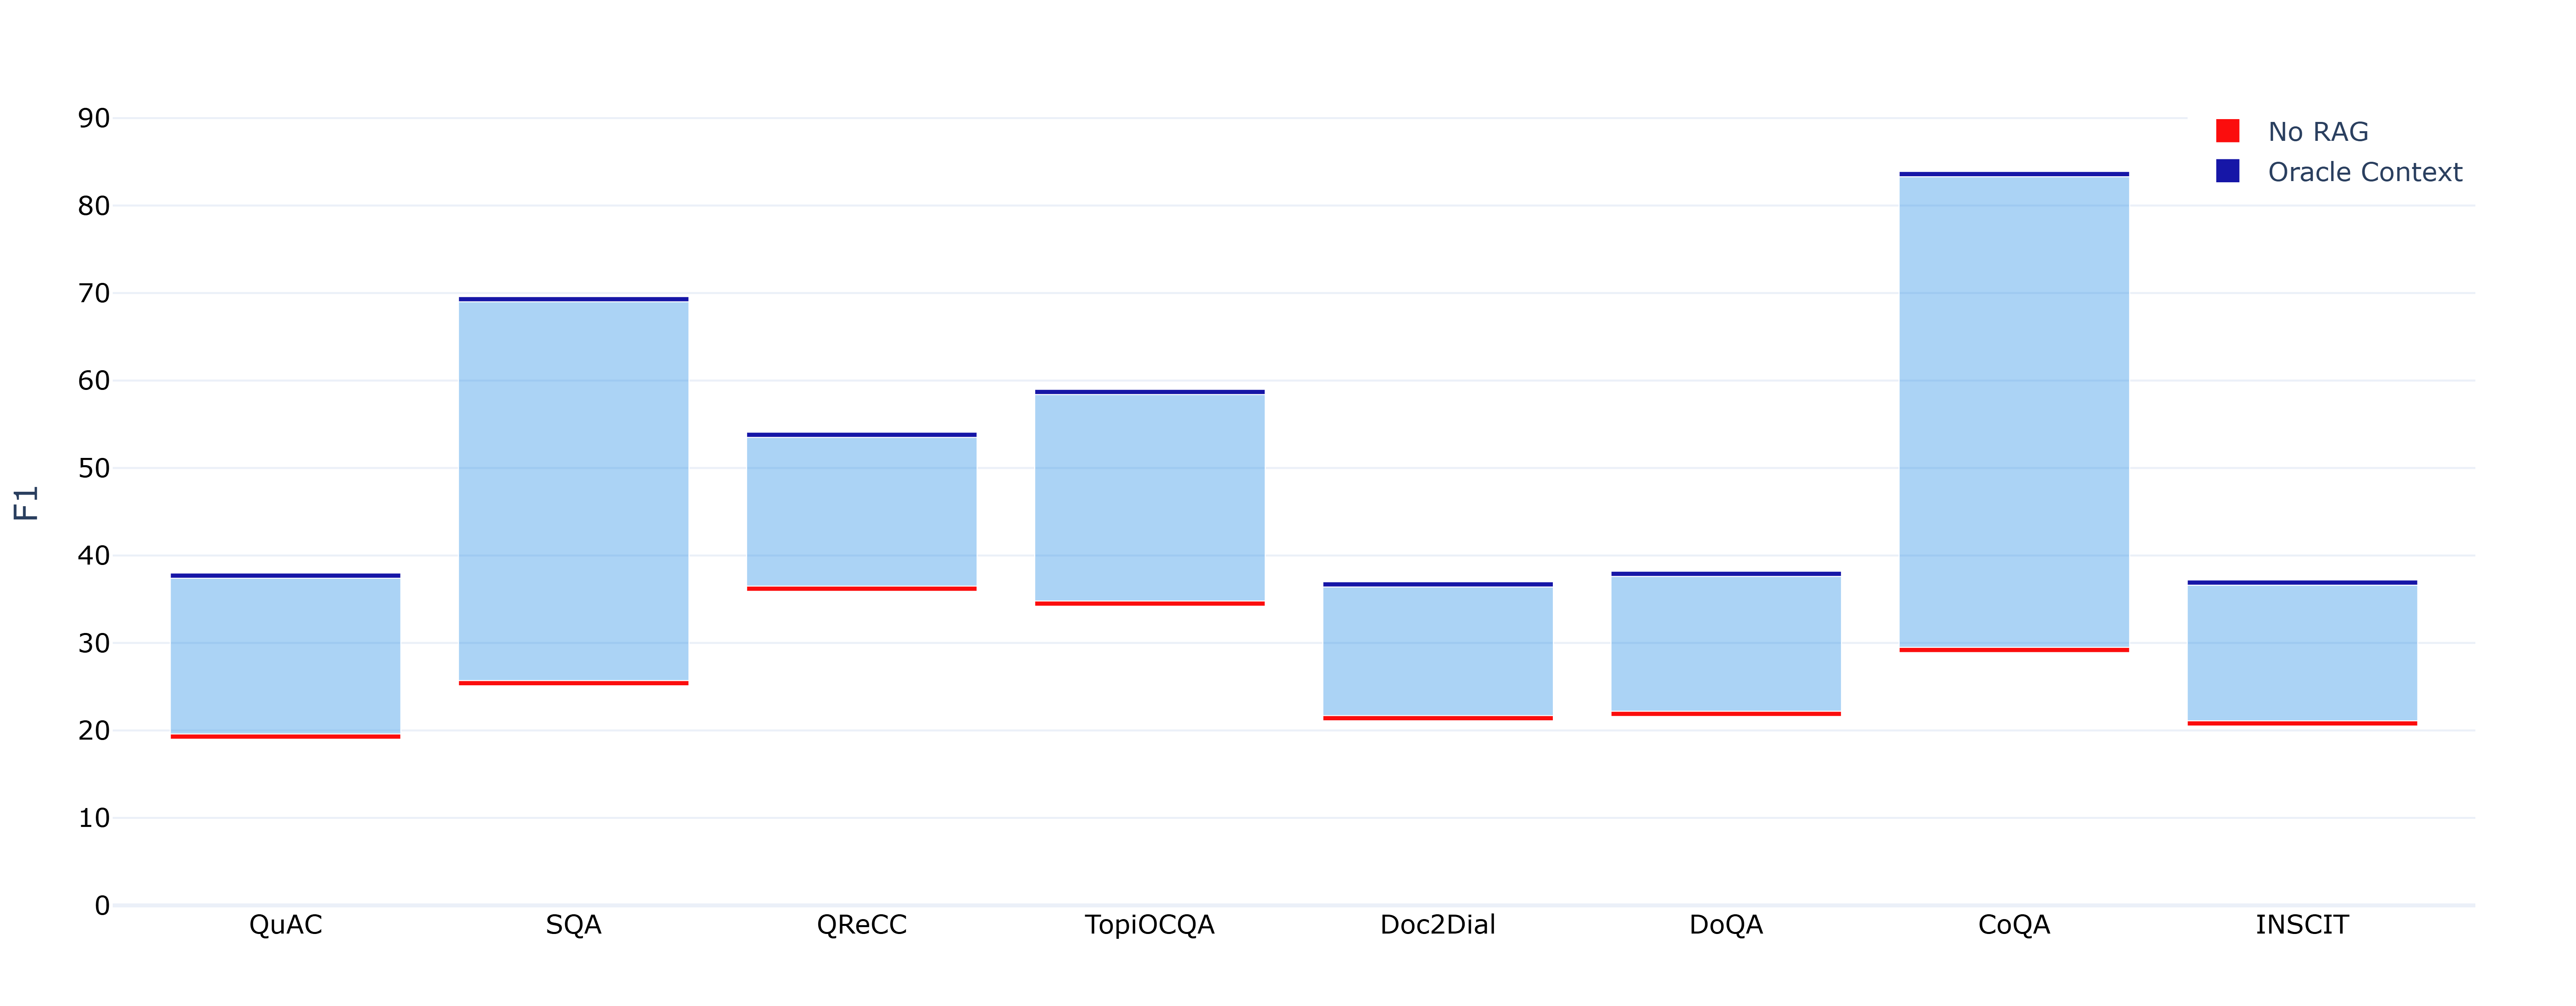
\includegraphics[width=\linewidth]{plots/f1_range_bars.png}
  \caption[Min-Max F1 Range]{Theoretical minimum and maximum ranges of F1 that can be achieved with the LLM. Minimum is achieved by \textit{No RAG} method, which retrieves no contexts, whereas the maximum is achieved by the \textit{Oracle Context} method, which directly uses the gold label context.}\label{fig:f1_min_max_range}
\end{figure*}


\subsection{Dataset Statistics} \label{sec:statistics}

In total, our analysis encompasses over \textbf{29,000} QA pairs and more than \textbf{245,000 } distinct contexts across multiple domains. As shown in Table~\ref{table:datasets}, the datasets exhibit significant structural variation. The ratio of context tokens to query tokens varies considerably across the different subsets, whereas the average question length remains relatively balanced (7--12 tokens). In contrast, answer and context lengths exhibit substantial variance: average answer lengths range from 4 tokens (CoQA) to 45 tokens (INSCIT), whereas average context lengths range from approximately 100 to 500 tokens. 
Table \ref{table:datasets} presents the answer lengths, which vary considerably, ranging from the more concise answers in the CoQA dataset to the lengthier explanations in INSCIT, which were already accounted for in the system prompts.
While longer contexts risk containing more distracting content and reducing generator performance, shorter contexts can be disadvantageous if they do not provide sufficient context. 
A larger number of total contexts, as in the QuAC, INSCIT, and TopiOCQA datasets, could complicate or delay context retrieval. 

\subsection{Dataset Analysis} \label{sec:preliminary analysis}
To assess whether the datasets are suitable for analysis and whether they theoretically benefit from RAG, we conducted a pre-study in which we queried each dataset with the model using no information and with all information about the query.
We evaluate two control settings to disentangle pre-trained knowledge from the effect of context: \textit{No RAG}, which queries the LLM without external context, and \textit{Oracle Context}, which provides only the ground-truth context and serves as an upper bound, as shown in Figure~\ref{fig:f1_min_max_range}. 
We define the \textit{Oracle Context} setup as the upper bound of the model, given the generator's ability to answer the question using the golden context. 
In contrast, the lower bound is the LLM’s performance without any context, independent of the pre-trained model's knowledge.

For most datasets, the ceiling F1 remains below 40\%, with overall values around 15–20\%, indicating room for improvements through retriever methods alongside additional performance bottlenecks. CoQA and SQA exhibit wider F1 ranges, facilitating more precise comparisons between retrieval methods.
Furthermore, except for QReCC and TopiOCQA, the LLM displays comparable internal knowledge across datasets. Because LLMs are trained on public data, the \textit{No RAG} setting provides a valuable proxy for assessing overlap between the dataset and pre-training or fine-tuning data.



% \begin{table*}[!th]
% \centering
% \resizebox{\textwidth}{!}{
% \begin{tabular}{l l|cc|cc|cc|cc||cc|cc||cc|cc}
% \toprule
% \multirow{4}{*}{\textbf{RAG Method}} & \multirow{2}{*}{} 
%   & \multicolumn{2}{c|}{\textbf{QuAC}}  
%   & \multicolumn{2}{c|}{\textbf{SQA}}  
%   & \multicolumn{2}{c|}{\textbf{QReCC}}  
%   & \multicolumn{2}{c|}{\textbf{TopiOCQA}}  
%   & \multicolumn{2}{c|}{\textbf{Doc2Dial}}  
%   & \multicolumn{2}{c|}{\textbf{DoQA}}  
%   & \multicolumn{2}{c|}{\textbf{CoQA}}  
%   & \multicolumn{2}{c}{\textbf{INSCIT}} \\
%   \cmidrule(lr){3-18} 
% & & \multicolumn{8}{c|}{Wikipedia} & \multicolumn{2}{c|}{Social Welfare} & \multicolumn{2}{c|}{StackExchange} & \multicolumn{4}{c|}{Mixed} \\
% \cmidrule(lr){3-4} \cmidrule(lr){5-6} \cmidrule(lr){7-8} \cmidrule(lr){9-10} 
% \cmidrule(lr){11-12} \cmidrule(lr){13-14} \cmidrule(lr){15-16} \cmidrule(lr){17-18} 
% & & F1 & MRR & F1 & MRR & F1 & MRR & F1 & MRR & F1 & MRR & F1 & MRR & F1 & MRR & F1 & MRR \\
% \midrule
% \textit{No RAG} & & 19.0 & - & 25.1 & - & 35.9 & - & 34.2 & - & 21.1 & - & 21.6 & - & 28.9 & - & 20.5 & - \\
% \textit{Oracle Context} & & 38.0 & 100 & 69.6 & 100 & 54.1 & 100 & 59.0 & 100 & 37.0 & 100 & 38.2 & 100 & 83.9 & 100 & 37.2 & 100 \\
% \hline
% \textit{Vanilla RAG} & & 25.4 & 35.3 & 43.8 & 66.1 & 36.5 & 36.6 & 33.9 & 8.7 & 26.3 & 49.0 & 36.2 & 92.0 & 58.3 & 72.5 & 19.2 & 8.0 \\
% \textit{Hybrid BM25} & & 27.5 & \textbf{44.6} & 45.6 & 53.8 & 37.4 & 37.4 & 34.0 & 9.4 & 27.7 & 51.0 & \textbf{36.9} & 84.8 & 67.3 & 76.6 & 19.1 & 8.1 \\
% \textit{Reranker} & & \textbf{29.2} & 41.6 & \textbf{51.3} & \textbf{71.0} & 36.0 & 35.3 & 34.2 & 9.8 & \textbf{28.7} & 54.0 & 36.7 & \textbf{93.1} & \textbf{74.7} & 78.9 & 19.1 & 9.5 \\
% \hline
% \textit{Query Rewriting} & & 20.8 & 35.3 & 38.1 & 66.1 & 32.5 & 36.4 & 26.9 & 8.7 & 21.6 & 49.0 & 27.6 & 92.0 & 47.5 & 72.4 & 16.7 & 8.0 \\
% \textit{HyDE} & & 26.2 & 42.0 & 38.0 & 65.3 & \textbf{42.2} & \textbf{49.0} & \textbf{43.5} & \textbf{25.1} & \textbf{28.7} & \textbf{57.5} & 35.4 & 90.9 & 71.3 & \textbf{86.6} & \textbf{25.9} & \textbf{25.2} \\
% \textit{HyDE + Reranker} & & 25.4 & 30.5 & 38.4 & 61.6 & 37.0 & 37.5 & 37.6 & 14.6 & 26.4 & 48.0 & 34.7 & 85.2 & 53.0 & 58.2 & 22.0 & 13.9 \\
% \textit{Summarization} & & 24.3 & 38.6 & 34.9 & 57.8 & 39.2 & 38.3 & 27.9 & 6.1 & 25.6 & 44.3 & 29.4 & 84.5 & 48.6 & 67.6 & 18.4 & 7.4 \\
% \textit{SumContext} & & 26.3 & 37.7 & 35.1 & 57.7 & 37.1 & 40.0 & 27.5 & 6.7 & 26.7 & 44.9 & 35.4 & 85.3 & 62.7 & 68.0 & 18.5 & 7.4 \\
% \bottomrule
% \end{tabular}
% }
% \caption{Overall performance (F1 and MRR@5) of RAG methods on all eight conversational QA datasets. F1 is used for the generator, and MRR@5 for retrieval performance. \textbf{Bold} values indicate the maximum for each column.}
% \label{tab:rag_f1_mrr_final}
% \end{table*}

\begin{table*}[!th]
\centering
\resizebox{\textwidth}{!}{
\begin{tabular}{l l|cc|cc|cc|cc||cc|cc||cc|cc}
\toprule
\multirow{4}{*}{\textbf{RAG Method}} & \multirow{2}{*}{} 
  & \multicolumn{2}{c|}{\textbf{QuAC}}  
  & \multicolumn{2}{c|}{\textbf{SQA}}  
  & \multicolumn{2}{c|}{\textbf{QReCC}}  
  & \multicolumn{2}{c|}{\textbf{TopiOCQA}}  
  & \multicolumn{2}{c|}{\textbf{Doc2Dial}}  
  & \multicolumn{2}{c|}{\textbf{DoQA}}  
  & \multicolumn{2}{c|}{\textbf{CoQA}}  
  & \multicolumn{2}{c}{\textbf{INSCIT}} \\
  \cmidrule(lr){3-18} 
& & \multicolumn{8}{c|}{Wikipedia} & \multicolumn{2}{c|}{Social Welfare} & \multicolumn{2}{c|}{StackExchange} & \multicolumn{4}{c|}{Mixed} \\
\cmidrule(lr){3-4} \cmidrule(lr){5-6} \cmidrule(lr){7-8} \cmidrule(lr){9-10} 
\cmidrule(lr){11-12} \cmidrule(lr){13-14} \cmidrule(lr){15-16} \cmidrule(lr){17-18} 
& & MRR & F1 & MRR & F1 & MRR & F1 & MRR & F1 & MRR & F1 & MRR & F1 & MRR & F1 & MRR & F1\\
\midrule
\textit{No RAG} & &  - & 19.0 & - & 25.1 & - & 35.9 & - & 34.2 & - & 21.1 & - & 21.6 & - & 28.9 & - & 20.5 \\
\textit{Oracle Context} & & 100 & 38.0 & 100 & 69.6 & 100 & 54.1 & 100 & 59.0 & 100 & 37.0 & 100 & 38.2 & 100 & 83.9 & 100 & 37.2 \\
\hline
\textit{Vanilla RAG} & & 35.3 & 25.4 & 66.1 & 43.8 & 36.6 & 36.5 & 8.7 & 33.9 & 49.0 & 26.3 & 92.0 & 36.2 & 72.5 & 58.3 & 8.0 & 19.2 \\
\textit{Hybrid BM25} & & \textbf{44.6} & 27.5 & 53.8 & 45.6 & 37.4 & 37.4 & 9.4 & 34.0 & 51.0 & 27.7 & 84.8 & \textbf{36.9} & 76.6 & 67.3 & 8.1 & 19.1 \\
\textit{Reranker} & & 41.6 & \textbf{29.2} & \textbf{71.0} & \textbf{51.3} & 35.3 & 36.0 & 9.8 & 34.2 & 54.0 & \textbf{28.7} & \textbf{93.1} & 36.7 & 78.9 & \textbf{74.7} & 9.5 & 19.1 \\
\hline
\textit{Query Rewriting} & & 35.3 & 20.8 & 66.1 & 38.1 & 36.4 & 32.5 & 8.7 & 26.9 & 49.0 & 21.6 & 92.0 & 27.6 & 72.4 & 47.5 & 8.0 & 16.7 \\
\textit{HyDE} & & 42.0 & 26.2 & 65.3 & 38.0 & \textbf{49.0} & \textbf{42.2} & \textbf{25.1} & \textbf{43.5} & \textbf{57.5} & \textbf{28.7} & 90.9 & 35.4 & \textbf{86.6} & 71.3 & \textbf{25.2} & \textbf{25.9} \\
\textit{HyDE + Reranker} & & 30.5 & 25.4 & 61.6 & 38.4 & 37.5 & 37.0 & 14.6 & 37.6 & 48.0 & 26.4 & 85.2 & 34.7 & 58.2 & 53.0 & 13.9 & 22.0 \\
\textit{Summarization} & & 38.6 & 24.3 & 57.8 & 34.9 & 38.3 & 39.2 & 6.1 & 27.9 & 44.3 & 25.6 & 84.5 & 29.4 & 67.6 & 48.6 & 7.4 & 18.4 \\
\textit{SumContext} & & 37.7 & 26.3 & 57.7 & 35.1 & 40.0 & 37.1 & 6.7 & 27.5 & 44.9 & 26.7 & 85.3 & 35.4 & 68.0 & 62.7 & 7.4 & 18.5 \\
\bottomrule
\end{tabular}
}
\caption{Overall performance (MRR@5 and F1) of RAG methods on all eight conversational QA datasets. MRR@5 is used for retrieval performance and F1 for the generator. \textbf{Bold} values indicate the maximum for each column.}
\label{tab:rag_f1_mrr_final}
\end{table*}


\section{Evaluation and Results} \label{sec:data}

This section outlines the experiments we conducted to investigate the effect of RAG methods on multi-domain conversational QA. Firstly, we describe the experimental setups, prompt design, and evaluation metrics used in the assessment in ~\Cref{subsec:setup,subsec:promptdesign,subsec:metrics}. This is followed by discussing the results for the retriever and generator, and followed by the analysis of the relation of retriever and generator performance in~\Cref{subsec:retriever_analysis,subsec:generator_analysis,subsec:interaction}. We further analyze the effect of the conversation turn and discuss the results in~\Cref{sec:ablation_studies,ch:6-discussion}.


\subsection{Experimental Setup}\label{subsec:setup}
We evaluated all advanced RAG methods across all eight datasets using the EncouRAGe~\cite{strich_encourage_2025} library with the Llama 3 8B Instruct model \cite{grattafiori_llama_2024}, selected for its strong language understanding and manageable computational requirements. Additionally, the results of Gemma 3 27b~\cite{kamath_gemma_2025} were added in the camera-ready version in Appendix~\ref{apx:gemma3} and align with all results.
%The model combines pre-training on large corpora with grouped-query attention \cite{ainslie_gqa_2023} and post-training instruction tuning via supervised fine-tuning and direct preference optimization for improved alignment with human instructions. 
Key parameters were set to ensure reproducibility and efficiency: temperature = 0, maximum output length = 1000 tokens, and context length = 40,000 tokens. 
We conducted multiple runs for each method but observed only negligible differences across runs, so we reported results for only one run per method and dataset. 
Inference was performed on an NVIDIA RTX A6000 GPU with 48 GB of memory. EncouRAGe~\cite{strich_encourage_2025} facilitated dataset and RAG method management, integrating \texttt{vLLM} \cite{kwon_efficient_2023} for efficient batched inference and MLflow for experiment tracking. External contexts were stored in the Chroma vector database \cite{chromateam_chroma_2025} using Sentence Transformers \texttt{all-MiniLM-L6-v2}~\cite{reimers_making_2020} embeddings and Cosine Similarity for semantic relevance, ensuring efficient retrieval and evaluation across all methods and datasets.




\subsection{Prompt Design} \label{subsec:promptdesign}
Our prompt strategy relies on a consistent zero-shot template, following ChatQA~\cite{liu_chatqa_2024}. The general system prompt instructs the model to prioritize retrieved context and dialogue history, strictly avoiding reliance on internal knowledge to reduce hallucinations. Variations in the prompt were limited to formatting constraints (e.g., extraction vs. generation) to match specific dataset targets; the full set of dataset-specific prompt templates is provided in Appendix~\ref{apx:expanded_prompts}.

% \subsection{Experimental Setup}

% This chapter presents the experimental study conducted to compare the performance of advanced RAG methods on multiple datasets of varying topics and formats. The experiment is built upon the plan laid out in the Chapter \ref{ch:4-methodology}, and starts with Section \ref{sec:implementation} outlining how the LLM model was setup for this design to be implemented. Section \ref{sec:preliminary analysis} continues with a discussion on the results that can be expected from the experiment, based on a preliminary analysis. Afterwards, Section \ref{sec:empirical analysis} continues by discussing the experiment results, laying out the performance expectations that were set, and examining whether the final results fit these predictions. Section \ref{sec:ablation studies} finishes by doing a deeper analysis of any datasets or RAG method that displayed irregular outcomes. 


% As mentioned in Chapter \ref{ch:4-methodology}, the implementation of the experimental study was carried out using the Python library EncouRAGe, with the Llama 3 8B Instruct model \cite{grattafiori2024llama}. This model was chosen since it exhibits stronger language understanding than Llama 2 models \cite{touvron2023llama2} or smaller Llama 3 models such as Llama 3.2 1B \footnote{https://ai.meta.com/blog/llama-3-2-connect-2024-vision-edge-mobile-devices/}, while requiring a more manageable level of computational resources than larger models such as the 70B or 405B \cite{grattafiori2024llama} models. This model is also the one used by \citet{liu2024chatqa} to test the ChatRAG-Bench datasets, so an easier comparison could be made between the results. 

% The Llama 3 models are developed using a \textbf{pre-training} stage which trains the model for next-token prediction using various text corpuses  This stage builds upon the Llama 2 models by employing a larger tokenizer with a vocabulary of 128K tokens resulting in a more time-efficient text input, improving inference speed using grouped-query attention (GQA) \cite{ainslie2023gqa}, which acts as a middle ground between multi-head and multi-query attention, and ensuring that self-attention does not get applied across multiple documents by using an attention mask. The \textit{Instruct} models add a \textbf{post-training} stage which uses a combination of supervised fine-tuning using a specially trained reward model and direct preference optimization (DPO) to improve human preference alignment and instruction following. 

% When setting up for the experiment, certain parameters of the model can be altered so they are better tailored to the task at hand while still keeping efficient computing. The \textit{temperature}, which controls how deterministic the model is and how much of a role randomness plays, was set to $0$ since reproducible results are necessary in order to have a fair comparison between the different RAG methods. The \textit{max\_tokens} parameter, that decides the maximum length of the generated answer, was set to $1000$ and the \textit{max\_model\_len}, which sets the maximum context length that the model can process, was set to $40000$.

% The use of the LLM was assisted by the NVIDIA RTX A6000 GPU, which is used to reinforce the heavy computational needs. The Ampere-based architecture is equipped with 48 GB of ECC GDDR6 memory and over $10,700$ CUDA cores, which makes it ideal for the large data processing and intensive inference needed for the experiment \cite{nvidia_rtx_a6000}.  


% \subsection{Encourage} \label{sec:encourage}

% To facilitate the management and execution of the various datasets and RAG methods, the EncouRAGe library \footnote{https://github.com/uhh-hcds/encourage} is integrated into the code following its accompanying template \footnote{https://github.com/pesc101/exp-template}. EncouRAGe is a modular and flexible framework, whose workflow is shown in Figure \ref{fig:encourage} that supports the RAG process by improving inference efficiency, storing results and metadata, and enabling the use of multiple RAG methods and evaluation metrics.


% EncouRAGe uses two important libraries (vLLM, MLflow) to streamline LLM inference and the monitoring of runs and results. vLLM \cite{kwon2023efficient} is an open-source, end-to-end LLM serving engine that aims to optimize key-value (KV) cache memory usage. KV cache memory is comprised of the key and value tensors necessary for the attention function in transformers, and since it expands and shrinks dynamically based on the request size, it can be prone to fragmentation and management complexity. vLLM introduces PagedAttention, an algorithm that divides the KV cache memory into blocks that hold a fixed number of key-value pairs. The more efficient memory management allows for the successful batching of large amounts of requests. MLflow \cite{zaharia2018accelerating} is also an open-source platform designed to streamline model deployment, experiment execution, and reproducibility. The main features used in EncouRAGe are in regard to experiment tracking, where the parameters of each experiment (RAG method, dataset name, LLM model, etc), along with the evaluation metrics, and the full table of the requests, contexts, and results. 


% Another important part of the RAG method is the vector database where all external contexts are stored and subsequently retrieved. The one used in this case is the open-source, embedding database Chroma \cite{chromadb} which has an easily accessible core API, made up of four main functions. A ChromaDB client is created, and the collection of contexts are added to it, along with the choice of \textit{embedding models} and \textit{distance} function. While Chroma supports a variety of different embedding functions, the default is the Sentence Transformers \cite{reimers2019sentence} \textbf{all-MiniLM-L6-v2} model, which maps words and sentences to 384-dimensional vector embeddings. The distance function is used to calculate the approximate nearest neighbors (ANN) to the query vector, thus finding the most relevant contexts, with \textit{Squared L2}, \textit{Inner Product}, and \textit{Cosine Similarity} available. The default distance function, Cosine Similarity, as shown below 
% \begin{equation}
%     \text{d} = 1 - \frac{\sum{A_i \times B_i}}{\sqrt{\sum{A_i^2}} \cdot \sqrt{\sum{B_i^2}}}
% \end{equation}
% will be used in the experiment since it places more focus on the vector's direction rather than its magnitude, thus giving priority to the texts semantic meaning. 

\subsection{Evaluation Metrics}\label{subsec:metrics}
For generators, we considered using F1, with F1 adopted as the primary metric to align with prior ChatRAG-Bench studies \cite{liu_chatqa_2024}. We selected the F1 Score from the SQuAD paper~\cite{rajpurkar_squad_2016} to balance token-level precision and recall, and, for datasets with multiple valid answers, we used the maximum score across references. Retriever performance was assessed using Recall@$k$, indicating whether the ground-truth context appears in the top-$k$ retrievals, and Mean Reciprocal Rank (MRR)~\cite{kantor_trec5_2000} for \textit{k} = 5, which emphasizes correct contexts ranked higher. These metrics together capture both the accuracy and ranking quality of retrieval, facilitating fair comparison across RAG methods.

% There are a variety of different evaluation metrics available in the EncouRAGe platform to evaluate the performance of both the generators and the retrievers. Among the generator evaluation metrics considered were BLEU \cite{papineni2002bleu}, GLEU \cite{napoles2016gleu}, ROUGE \cite{lin2004rouge} and F1, whereas Recall@k and Mean Reciprocal Rank (MRR) were both used for assessing the retrievers performance.

% \subsubsection*{Generator evaluation metrics}

% The F1 score is calculated using the harmonic mean of the token-based precision and recall,  
% \begin{equation}
%     \text{F1} = \frac{\text{Precision} \times \text{Recall}}{\text{Precision} + \text{Recall}}
% \end{equation}
% thus creating a balance between correctness and completeness. BLEU \cite{papineni2002bleu}, first used for assessing machine translation, is based on the geometric average of generated answers n-gram precisions $p_n$ with an added brevity penalty (BP) for generations shorter than the reference answer length. This is shown in 
% \begin{equation} 
%     \text{BLEU} = BP \times \exp\left(\sum_{n=1}^{N} w_n \cdot \log p_n\right) 
% \end{equation}
% with $N$ and $w_n$ representing the size and weights of the n-grams respectively. Using this as a foundation, the GLEU \cite{napoles2016gleu} metric keeps the n-gram comparison but instead using the harmonic mean of F1. On the contrary, ROUGE \cite{lin2004rouge} is more recall-oriented and is split into multiple varieties, with ROUGE-L used to determine the longest common subsequence between the generated and reference answer, and ROUGE-N being calculated as follows:
% \begin{equation}
%  \text{ROUGE-N} = \frac{\sum_{\text{gram}_n \in \text{Ref}} \text{Count}_{\text{match}}(\text{gram}_n)}
% {\sum_{\text{gram}_n \in \text{Ref}} \text{Count}(\text{gram}_n)}
% \end{equation}
% where $Count(gram_n)$ is the total number of n-grams in the reference answer and $Count_{match}(gram_n)$ is the amount of n-grams occurring in both answers. 

% Ultimately, since the original paper \cite{liu2024chatqa} that introduced and experimented with the ChatRAG-Bench dataset collection focuses its results on F1, in order to have a fair comparison this study will also use F1 as the main evaluation metric to compare the generated answer to the reference answer. As mentioned in \ref{sec:data}, some of the datasets have multiple correct answers, so similar to it is handled in their respective papers \cite{rajpurkar2016squad, reddy2019coqa, choi2018quac}, the F1 score will be separately calculated for each possible answer, with the one possessing the maximum score being chosen.

% \subsubsection*{Retriever evaluation metrics}

% The performance of the retriever is evaluated on a two-pronged approach: first, does the retriever fetch the correct context, and second, is the correct context ranked higher than the others. Recall@k is a binary metric which outputs a $1$ if it determines that the ground truth context appears within the top \textit{k} retrievals, or a $0$ otherwise. MRR \cite{kantor2000treck} emphasizes the priority of the correctly retrieved context by averaging the reciprocal of their ranking, as shown below, 
% \begin{equation}
%     \text{MRR} = \frac{1}{N} \sum_{n=1}^{N} \frac{1}{rank_i} 
% \end{equation}
% where $N$ is the total number of retrieved contexts, and $rank_i$ representing the rank of the ground truth context(s). In the experiment study, both metrics will be essential in order to determine how significant the effect of the ranking is on the performance and to ease the comparison of the different RAG methods. 

\begin{figure*}[tb]
  \centering
  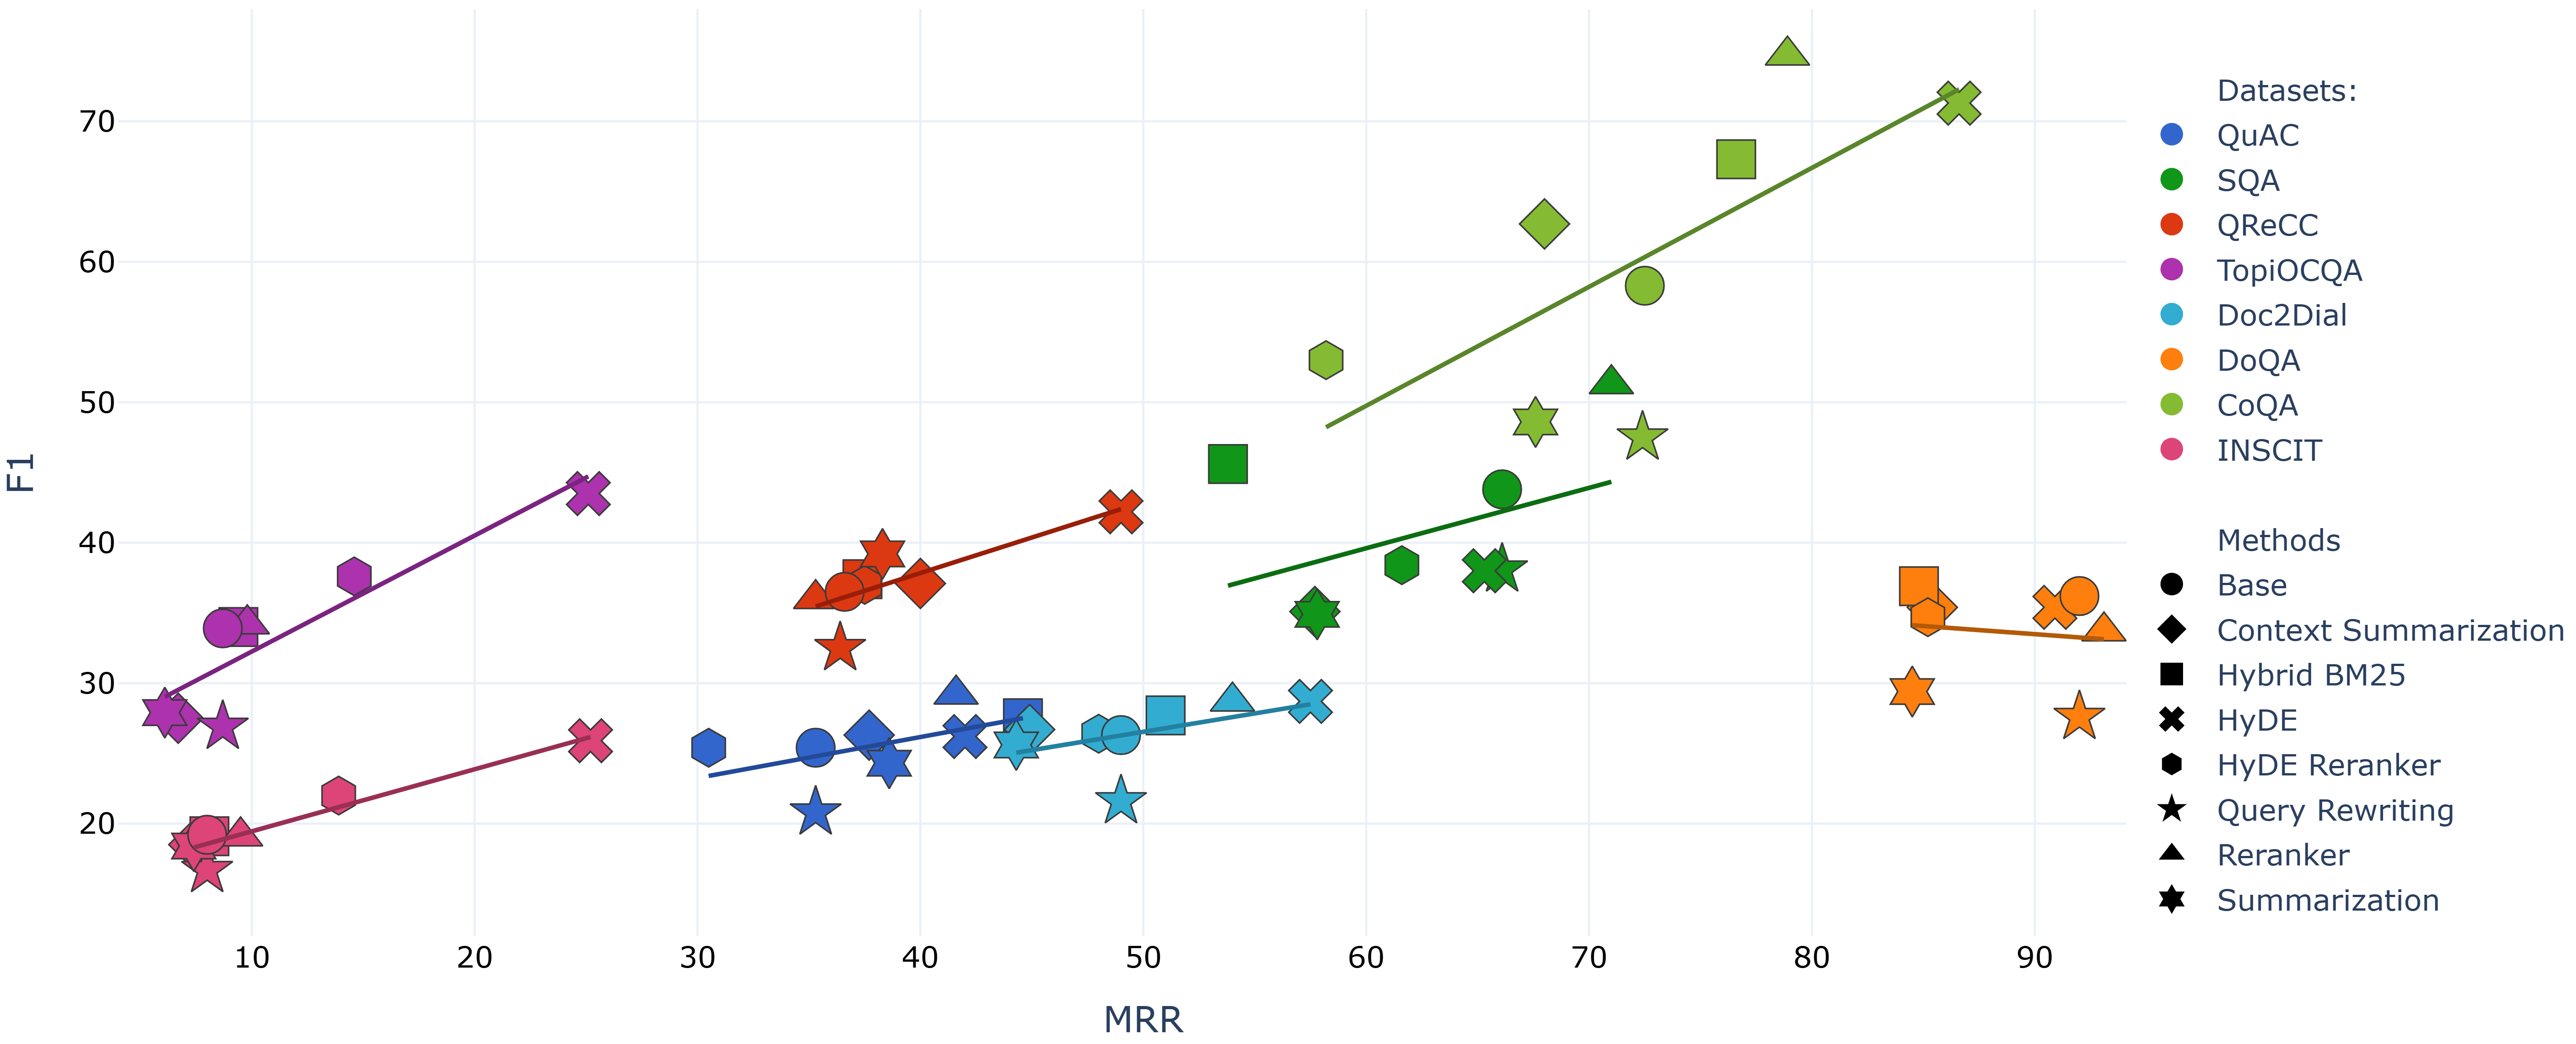
\includegraphics[width=\linewidth]{plots/scatter_plot_dataset_methods_regression.png}
  \caption[Distribution of F1 and MRR by method and dataset]{Relationship between retriever (MRR@\textit{5}) and generator (F1) performance for each dataset and method.}  \label{fig:scatter_f1_mrr_method_dataset}
\end{figure*}


\subsection{Retrieval Results}\label{subsec:retriever_analysis}
Table~\ref{tab:rag_f1_mrr_final} presents the results of the generator and retriever for each of the RAG methods. We also report Recall@\textit{1} and Recall@\textit{5} for each approach in Appendix~\ref{apx:retrieval}.
In terms of MRR@\textit{5} performance, for all datasets except for SQA~\cite{iyyer_searchbased_2017} and DoQA~\cite{campos_doqa_2020}, the combination of sparse and dense encoders in \textit{Hybrid BM25} leads to better results than \textit{Vanilla RAG}. This effect is also visible for the \textit{Reranker}.

Among the advanced RAG methods, \textit{HyDE} ranks clearly ahead, achieving the best performance on five of eight datasets. 
It is important to highlight that for INSCIT, \textit{HyDE} triples the performance of \textit{Vanilla RAG}.
The two summarization methods yielded poor retrievals, suggesting that summarization may remove crucial contextual information.
Dataset-wise, the MRR@\textit{5} values were highest in the DoQA and CoQA datasets and were significantly lower in INSCIT and TopiOCQA, which are analyzed further in Section \ref{sec:ablation_studies}.

\subsection{Generator Results}\label{subsec:generator_analysis}
Table~\ref{tab:rag_f1_mrr_final} shows that \textit{Hybrid BM25} consistently achieves slightly higher F1 scores than \textit{Vanilla RAG} across all datasets. Consistent with the retriever results, \textit{HyDE} emerges as the strongest approach, attaining the highest performance on four of the eight datasets and highlighting its effectiveness for conversational QA. This advantage is particularly evident on TopiOCQA, where \textit{HyDE} improves the F1 score by 9.6\% over \textit{Vanilla RAG}. In contrast, the performance of \textit{Query Rewriting} is highly dataset-dependent and falls substantially below \textit{No RAG} on the INSCIT, QReCC, and TopiOCQA datasets, where MRR scores are also below average. This may point to differences in conversational structure, such as larger topic shifts or longer dependency chains, that render these datasets less effective for this method. Finally, for summarization methods, incorporating the original conversational context yields only marginal improvements except for DoQA and CoQA.

\subsection{Relationship of Retriever and Generator}\label{subsec:interaction}
% The relationship of retrieval and generation is illustrated in Figure~\ref{fig:scatter_f1_mrr_method_dataset}. 
% Overall, the results indicate that F1 and MRR are correlated, suggesting that better retrieval is expected to yield higher answer quality. This is especially evident in INSCIT, TopiOCQA, CoQA, and SQA, where \textit{HyDE} and \textit{HyDERanker} confirm this trend.

% In contrast to this, are the results of QuAC and Doc2Dial. The differences between the methods are not as big as for the other datasets, but they show only slighty improvements. That a high MRR does not automatilly means high F1 Score is espically visible for DoQA, where the MRR is over 90\% but the generator seems to have problem to achive perofrmance above 40\%.

Figure~\ref{fig:scatter_f1_mrr_method_dataset} illustrates the relationship between retrieval and generation, with a fitted linear regression line summarizing the overall performance trend. Overall, F1 and MRR are positively correlated, indicating that stronger retrieval generally leads to higher answer quality, particularly on INSCIT, TopiOCQA, CoQA, and SQA, where \textit{HyDE} and \textit{HyDE Ranker} follow this trend. For CoQA and SQA, \textit{Reranker} appears to perform best, yielding the highest overall results on these datasets.

In contrast, QuAC and Doc2Dial show only marginal differences across methods, and the correlation is weaker. This disconnect is most pronounced for DoQA, where MRR exceeds 90\% but F1 remains below 40\%, highlighting that strong retrieval does not necessarily translate into strong generation. 

Furthermore, Spearman's  $\rho$ in Table~\ref{table:spearman} illustrates that most datasets have a relatively high correlation between the F1 and MRR values. The only exceptions being SQA and DoQA, which show weak or even negative correlations, suggesting that the two metrics capture different aspects of method performance.

These differences can be attributed to dataset specific problems, particularly relating to variations in answer formats. Answer conciseness is associated with overall high F1 scores, particularly when comparing CoQA's short responses against QReCC and INSCIT's longer, more in-depth answers, which are more challenging to match. 

\begin{table}[!htbp]
\centering
\begin{tabular}{l | l}
\toprule
\textbf{Subset} & \textbf{$\rho$} \\
\midrule
QuAC         & 0.620 \\
SQA          & 0.383 \\
QReCC        & 0.857 \\
TopiOCQA     & 0.874 \\
Doc2Dial     & 0.687 \\
DoQA         & -0.157 \\
CoQA         & 0.762 \\
INSCIT       & 0.788 \\
\bottomrule
\end{tabular}
\caption{Illustration of the Spearman's rank correlation coefficient ($\rho$), calculated for the F1 and MRR values for each dataset.}
\label{table:spearman}
\end{table}

The answer content can also heavily influence the performance, such as the social welfare answers of Doc2Dial, which rely on specific case details (user eligibility, personal details) and predetermined scripts, with many answers taking the form of follow-up questions requesting further information. Similarly, the forum-based DoQA dataset contains many informal responses in which respondents draw on personal knowledge rather than relying solely on the provided context. Additionally, the sensitive nature of certain DoQA queries leads to the generator refusing to respond, on the grounds that it cannot provide legal advice or discuss topics relating to violence or weaponry. 





% \subsubsection{Analysis of high-performing RAG methods}
% A look into the overall F1 and MRR values shown in Table \ref{table:full_f1_mrr}, showed that the RAG methods, which showed the most accurate retrieval, did not necessarily always translate to the highest F1 values. The standout method in both the MRR and Recall retrieval metrics was HyDE, which, to restate, generates a document that would hypothetically answer the prompt question, which is then used to map to the ground truth contexts during retrieval. Evidently, this proves to be a successful approach, since it combines the supplementary information given by the contexts, while making sure it is tailor-made only to the latest question instead of the topic in general. The second best performer was Hybrid BM25, which integrates both dense and sparse retrieval, thus searching for both lexical and semantic matches. This shows that the contexts of some datasets have quite a considerable lexical overlap with the query and conversation history, and using only dense retrievers might lead to more generalized terms being searched and less priority given to those using the exact terminology. 

% Transitioning to the F1 values, it could be assumed that HyDE and Hybrid BM25 are among the highest performers, but that is only the case for the latter, which, on average, has the second-highest F1 performance across all datasets. On the other hand, the former achieved much lower scores, despite its high retrieval rate. This shows that Hybrid BM25 works as a good middle-ground between the two metrics, demonstrating the effectiveness of the sparse encoder in both precision and recall. The top performer in terms of answer quality across five out of the eight datasets was the Reranker method, which showed relatively moderate retrieval scores.

% \begin{figure}[tb]
%   \centering
%   \includegraphics[width=\linewidth]{plots/recall_comp.png}
%   \caption[Recall@k comparison between HyDE and Reranker methods]{Plot showing the comparison of Recall values for the HyDE and Reranker methods, across the datasets where Reranker has the highest F1 performance. Recall@1 measures whether the correct context was retrieved in the first position whereas Recall@5 measures whether it occurs in the top 5 contexts. }\label{fig:recall_comp}
% \end{figure}

% To take a closer look at why the Reranker could outperform HyDE, although its MRR scores are higher, Recall@k could also be analyzed, which shows whether the ground truth contexts appear in the top \textit{k} scores, the full scores of which can be seen in Appendix \ref{app:results}. Figure \ref{fig:recall_comp} shows a comparison between Recall@1 and Recall@5, and it can be seen that while Reranker has a lower chance of finding the correct context among all the retrieved ones, when it does find it, it is more likely to boost it up to the highest placement. Since each prompt has only one ground truth context, not much can be analyzed about the contexts that do not contain the correct answer but are topically related, but it is conceivable that Reranker might also place these higher, thus reducing the amount of unrelated contexts. 

% \begin{figure*}[tb]
%   \centering
%   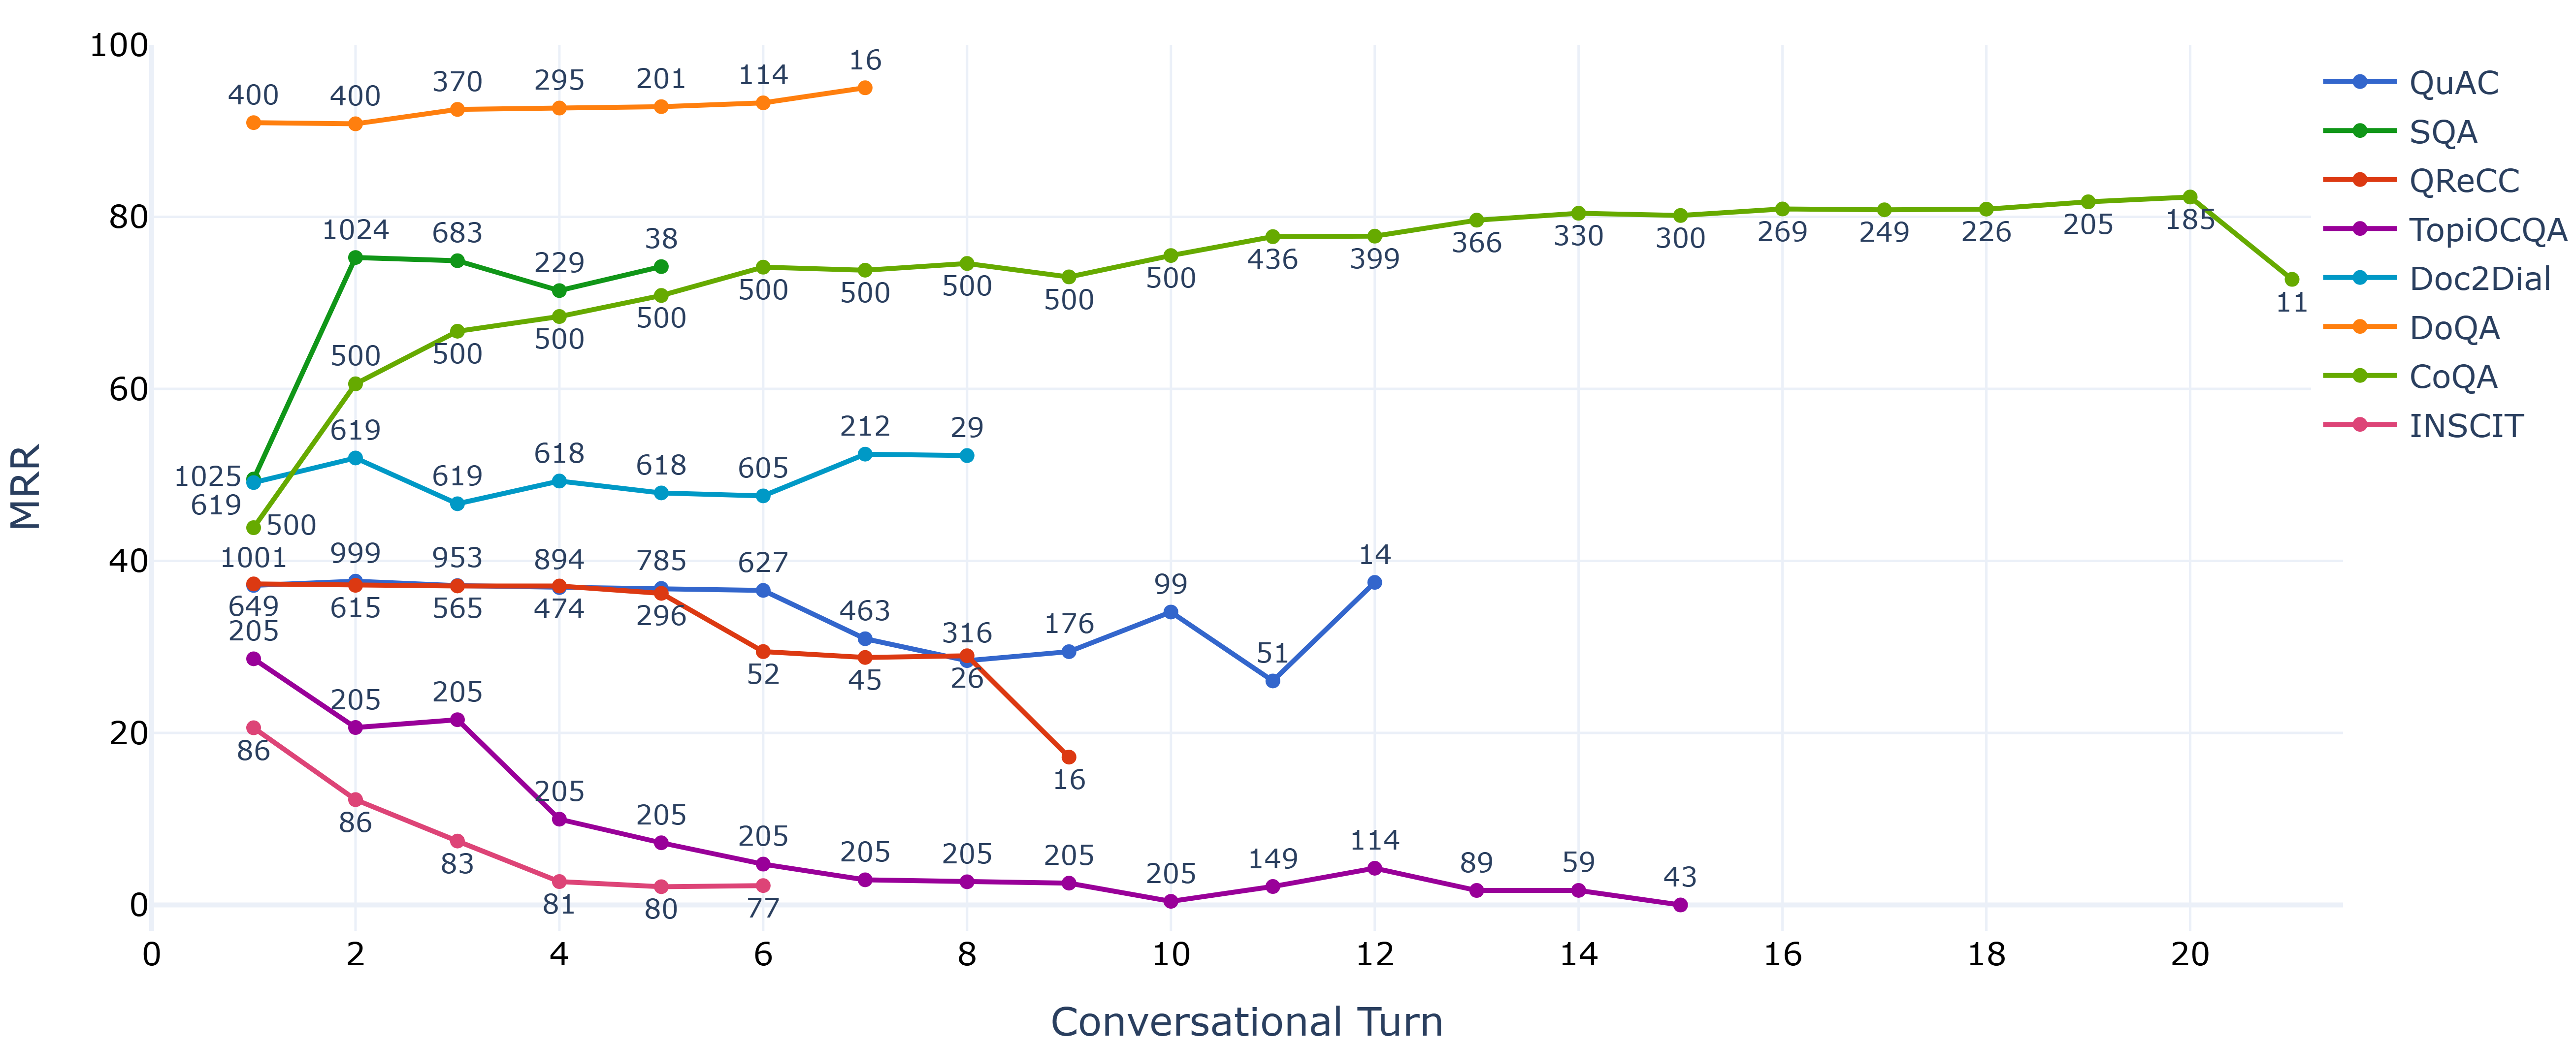
\includegraphics[width=\linewidth]{plots/conv_mrr.png}
%   \caption[MRR development over conversation turns]{Graph showing how the MRR performance changes over each conversation turn. }\label{fig:conv_mrr_lim}
% \end{figure*}

% \subsubsection{Analysis of low-performing datasets}

\begin{figure*}[tb]
  \centering
  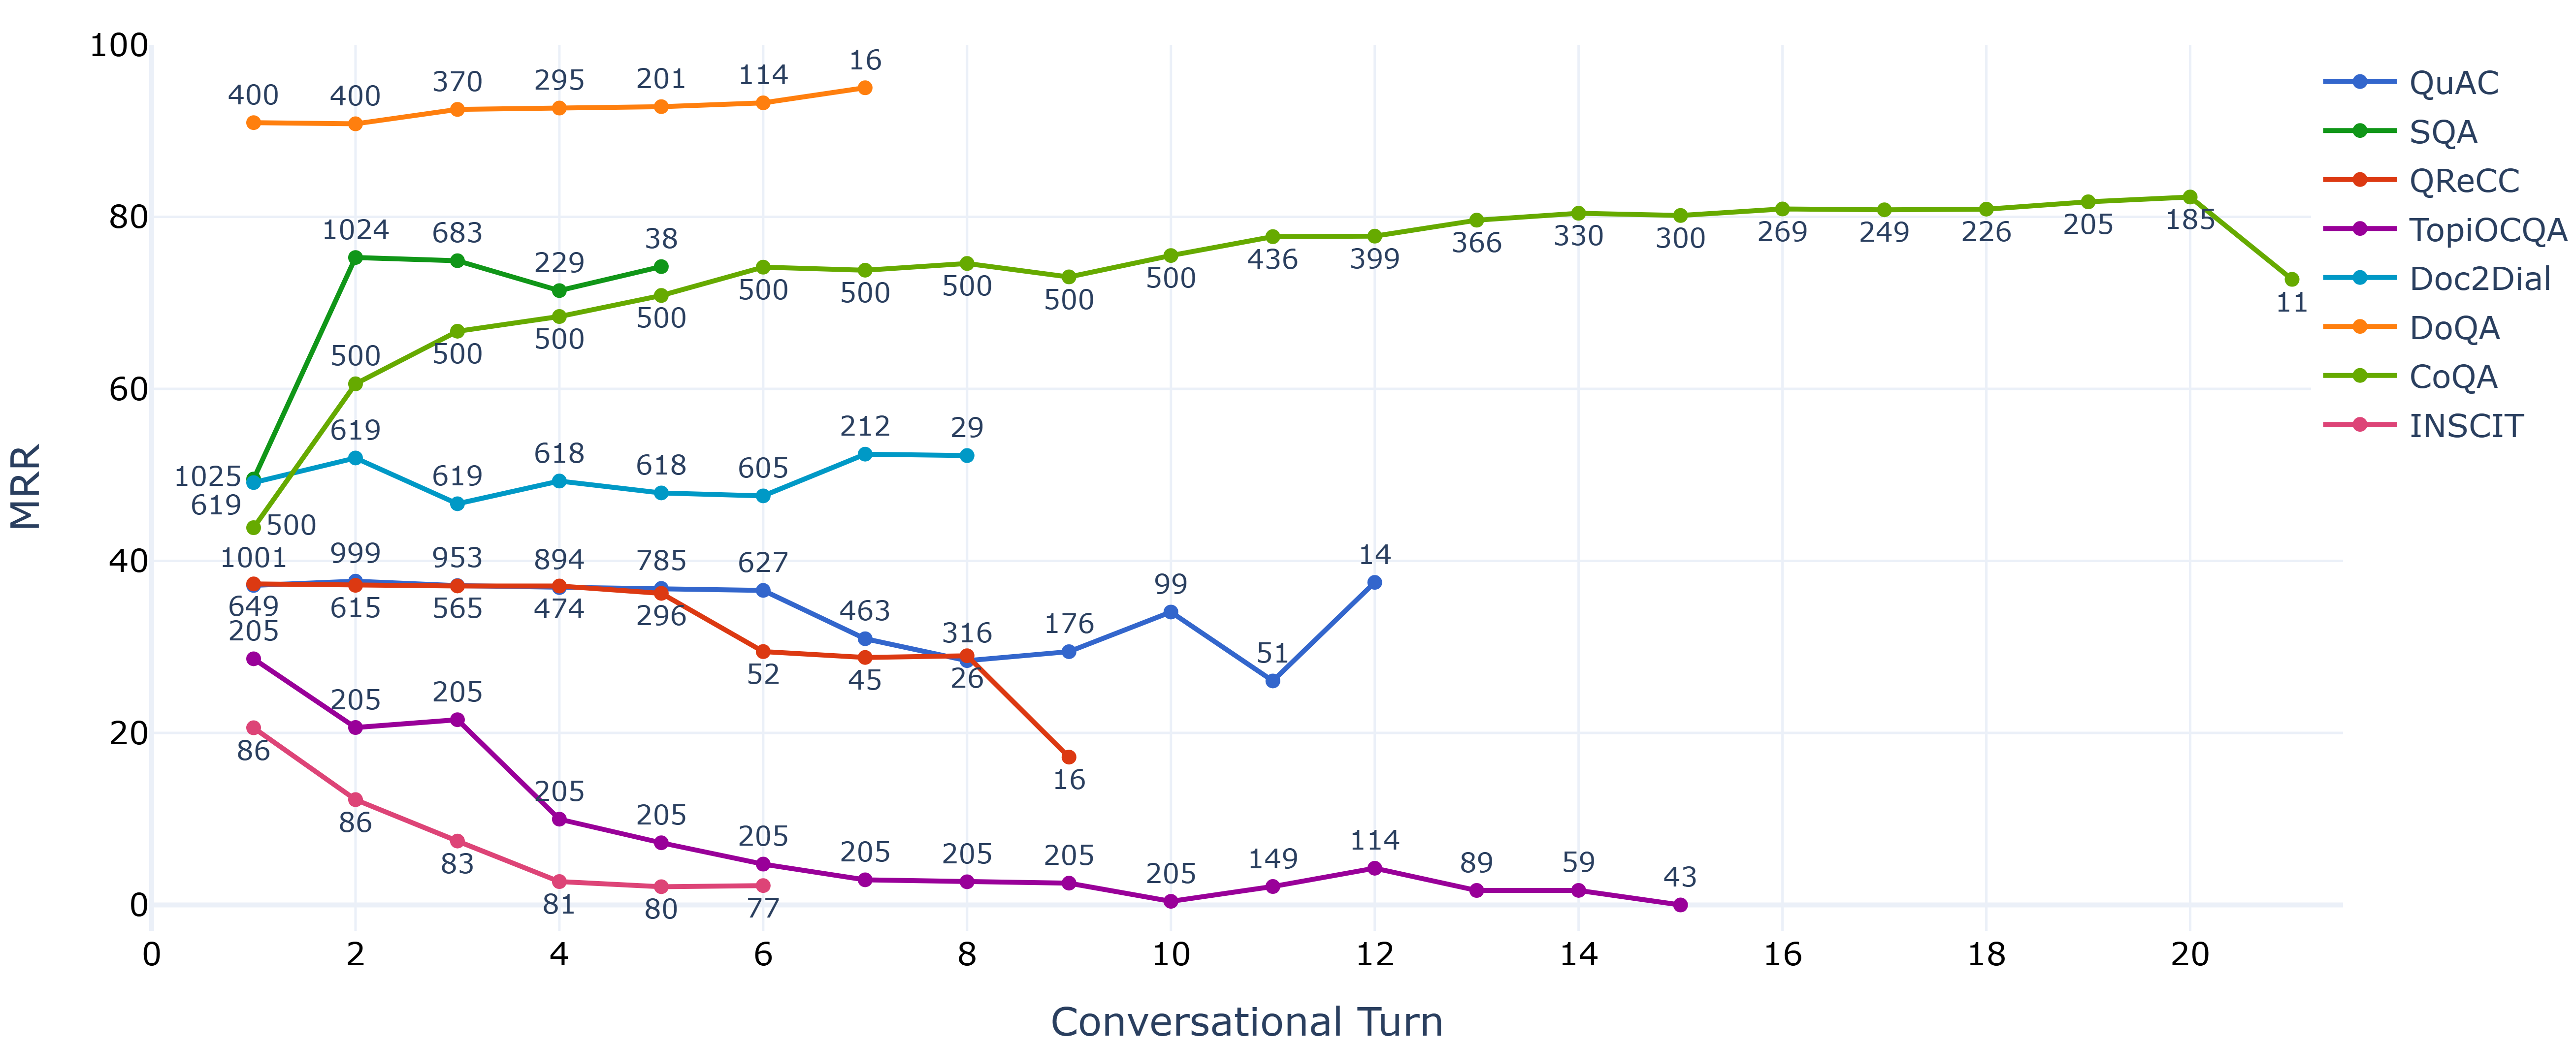
\includegraphics[width=\linewidth]{plots/conv_mrr.png}
  \caption[MRR development over conversation turns]{MRR performance across conversational turn for each dataset using \textit{Vanilla RAG}. The annotations indicate the number of samples per turn for each dataset.}\label{fig:conv_mrr_lim}
\end{figure*}

\subsection{Ablation Study} \label{sec:ablation_studies}
To further understand the effect of RAG on conversational QA, we examine retrieval performance across conversational turns in Figure~\ref{fig:conv_mrr_lim}. We compute MRR and F1 Score by turn position to identify trends in retrieval performance and present the F1 results in Appendix~\ref{apx:conv_f1}.
We find mixed results for all eight datasets. It is expected that INSCIT and TopiOCQA exhibit low performance that steadily decreases with the number of turns, primarily due to the high Ctx/Q ratio, as shown in Table~\ref{table:datasets}. This generally leads to low retrieval performance, and both datasets are designed to support topic and interaction entity switching.

In contrast, CoQA and SQA benefit from more context and improve performance with each turn, indicating that, when the context is consistent, more information leads to better retrieval performance. We found in addition that for QReCC, QuAC, DoQA, and Doc2Dial, all datasets seem to show no difference regarding the number of conversational turns til turn 5. There, we find that QReCC and QuAC show performance decreases that warrant further investigation in future work.

Overall, the results suggested that when the context is consistent, retrieving it from the entire conversation is beneficial; however, when questions are topic-switching or when other entities are interacting, this approach can decrease retrieval performance. We therefore recommend that calculating the similarity between queries and conversational histories can benefit retrieval performance.




% As seen in Table \ref{tab:rag_f1_mrr_final}, no RAG methods showed any significant performance increases for the INSCIT, QReCC, and TopiOCQA datasets. 
% An analysis was done into whether this could be attributed to the number of conversation turns. A longer conversation history poses as a double-edged sword, since it can add much-needed contextual information, especially in the case of ambiguously phrased questions, but the slight topic changes can lead to attention being diverted away. It is expected that for each dataset, the point where the drawbacks start to outweigh the benefits differs.

% The MRR results for Base RAG were analyzed across each conversation turn, as shown in shown in Figure \ref{fig:conv_mrr_lim}, revealing a sharp drop for TopiOCQA, QReCC, and INSCIT with each ensuing question. This indicates that an extensive conversation history can make it more difficult to fetch the correct context, especially since these datasets an above average number of total contexts. The opposite trend occurs for the SQA, DoQA, and CoQA datasets, with the additional QA history increasing the retrieval accuracy. The remaining datasets, QuAC and Doc2Dial, exhibit relatively consistent results throughout.

% The analysis looked into the F1 and MRR results of these three datasets when using the Base RAG implementation, since it was planned to be used as a control group, and did surpassed the No RAG performance on the other datasets. Firstly, the F1 results of the datasets were examined, as seen in Figure !!!, and as expected, in the case of QReCC and TopiOCQA, they steadily decrease as the conversation history increases. Even at the earliest points in the conversation history, the performance is still comparable to the No RAG performance, which indicates that the issue could lie with the context retrieval. 

% The performance of the retriever, shown in Figure \ref{fig:conv_mrr_lim}, reveals that for QReCC and INSCIT, the MRR values drop sharply after the first couple of questions. This shows that the larger conversation history does make it more difficult to fetch the correct retrieval, especially for these datasets which have upward of $22,000$ contexts. This means that the distraction that the conversation history creates during the retrieval outweighs any benefits that this contextual information might provide. For TopiOCQA, the drop is less steep, but the consistent, low MRR is to be expected given the over $169,000$ contexts, which would increase the likelihood of related but inaccurate contexts being fetched. In both figures, a small uptick in the F1 and MRR values is seen toward the higher end of the question amount, which could be attributed to anomaly cases, since they are far from the average conversation lengths.

%\subsubsection{Summarization versus Context Summarization}

% Subsection \ref{subsec:summarization} discussed the design of the Summarization and Context Summarization methods, which begin similarly by making the LLM generate more concise contexts but later differ, with the former using the altered contexts in the final prompts and the latter using the original versions. The question arose as to how these two methods would perform with the datasets and whether the use of different contexts would affect said performance. Table \ref{table:sum_mrr} shows the correctness of the retriever as measured with MRR, which, as expected, is quite similar, since both techniques use the same retrieval process. The values only differ by a few percent, which is well within the bounds of random error, and could be due to noise. 

% \begin{table*}
% \scriptsize
% \begin{center}
% \begin{tabular}{ c | c | c | c | c | c | c | c | c }
% \toprule
% & CoQA & Doc2Dial & DoQA (avg)& INSCIT & QReCC & QuAC & SQA & TopiOCQA  \\
% \midrule
% Summarization & 0.051 & 0.071 & 0.313 & 0.054 & 0.197 & 0.106 & 0.058 & 0.036 \\
% Context Summarization & 0.046 & 0.069 & 0.316 & 0.055 & 0.201 & 0.103 & 0.055 & 0.039 \\
% \bottomrule
% \end{tabular}
% \end{center} 
% \caption[Summarization comparison of MRR values]{Table showing the difference of the MRR values between the Summarization and Context Summarization values.} 
% \label{table:sum_mrr}
% \end{table*}

% \begin{table*}
% \scriptsize
% \begin{center}
% \begin{tabular}{ c | c | c | c | c | c | c | c | c }
% \toprule
% & CoQA & Doc2Dial & DoQA (avg)& INSCIT & QReCC & QuAC & SQA & TopiOCQA  \\
% \midrule
% Summarization & 0.276 & 0.202 & 0.215 & 0.208 & 0.361 & 0.189 & 0.256 & 0.34 \\
% Context Summarization & 0.277 & 0.203 & 0.217 & 0.209 & 0.361 & 0.189 & 0.255 & 0.339 \\
% \bottomrule
% \end{tabular}
% \end{center} 
% \caption[Summarization comparison of F1 values]{Table showing the difference of the F1 values between the Summarization and Context Summarization values.}
% \label{table:sum_f1}
% \end{table*}

% It is worth noting that even the F1 values were very similar between the two methods, as shown in Table \ref{table:sum_f1}, despite their differences. Through these results, the effect of the summarized or non-summarized context is unclear. One possibility is that both versions contribute a similar amount of contextual information, thus the negligible performance difference between the two. Another explanation could be that the fault lies in the retriever, which is supported by the relatively low MRR scores, and the fact that the F1 values resemble those of the No RAG method. Essentially, the LLM is not getting sufficient contextual information and is instead relying on its internal knowledge to answer the question. 

% The summarization process is handled by the LLM, which condenses the contexts, and while the prompt can be finetuned to a certain level, this process cannot be fully controlled. Therefore, while the contexts of some datasets may benefit by the removal of tangential information, this does not seem to be the case for the datasets looked at in this experiment. 



\subsection{Discussion}\label{ch:6-discussion}%
This section examines whether conclusive findings were obtained and, if so, how they could inform future studies in Conversational QA or RAG.  We showed in our preliminary analysis that adding ground-truth context boosted performance by 15–50\%, providing a ceiling for RAG methods and a baseline for weaker ones. About half of the RAG methods performed on par with \textit{No RAG}, showing that inefficient pipelines either retrieve irrelevant contexts or fail to rank the ground-truth context highly enough.

% The addition of ground-truth context was shown to significantly improve performance, with gains ranging from 15\% to 50\%. The preliminary analysis, conducted beforehand, provided a useful ceiling for the expected values from the RAG methods, and the floor values were used to compare the lower-performing methods. Approximately half of the RAG methods yielded results comparable to \textit{No RAG}, even with added contexts, indicating that, in most cases, an inefficient RAG pipeline performs no better than \textit{No RAG}. A poor RAG pipeline may retrieve irrelevant contexts that could distract the LLM, or may not be able to elevate the ground-truth context to a sufficiently high position. 


As observed in the experiments, the results varied considerably across datasets and RAG methods, making it difficult to draw a unified conclusion. For F1, the top three methods were \textit{Reranker}~\cite{glass-etal-2022-re2g}, \textit{Hybrid BM25}~\cite{gao_complement_2021}, and \textit{HyDE}~\cite{gao_precise_2023}, respectively, indicating that \textit{Vanilla RAG}~\cite{lewis_retrievalaugmented_2020} was clearly outperformed across all datasets. Therefore, in one respect, the two advanced methods are recommended as superior alternatives in terms of performance. 
    
In contrast, it is essential to examine how the advanced RAG methods affect computational complexity and runtime overhead relative to \textit{Vanilla RAG.} To calculate relevance scores, \textit{Reranker} retrieves a larger number of candidate contexts, which are then passed through a cross-encoder. On the other hand, \textit{Hybrid BM25} adds a sparse retrieval function to the existing dense retrieval. Overall, although both methods are computationally simple, the experiment runs indicate that the double-retrieval process and score calculation of \textit{Hybrid BM25} result in slightly longer runtimes. 
While \textit{Vanilla RAG} does not achieve the highest overall performance, its high F1 scores and straightforward implementation make it a worthwhile baseline. Since the advanced methods do not deviate substantially from the baseline computationally, they also provide a valuable reference for estimating the potential performance of other advanced RAG methods. 

When examining the impact of dataset characteristics, the preliminary analysis revealed a substantial difference in the model's internal knowledge of specific dataset topics or formats. This is evident in the F1 range difference between Doc2Dial~\cite{feng_doc2dial_2020}, centered on specialized, open-ended questions in comparison to the factoid-style questions of CoQA~\cite{reddy_coqa_2019}. The total number of contexts significantly affected the retriever's performance by reducing the likelihood of finding the correct context.


\section{Conclusion} \label{sec:conclusion}

In this paper, we presented a systematic empirical study of vanilla and advanced RAG methods across eight multi-turn conversational QA datasets. Our evaluation, which accounted for both retriever effectiveness and generator quality, revealed that robust yet straightforward techniques, such as \textit{Reranker} and \textit{Hybrid BM25},  consistently outperform \textit{Vanilla RAG} across all evaluated domains. Among the advanced techniques studied, the HyDE method proved the most effective for enhancing retrieval performance, whereas the \textit{Reranker} approach was most successful at improving final answer quality. For future research, the results highlight that performance improvements can be achieved without inflating the computational complexity, emphasizing the need to prioritize retrieval strategies over resource-intensive scaling. 

Furthermore, our analysis of conversational turns demonstrated that the impact of dialogue depth varies substantially across datasets, reflecting their distinct structures. While some settings benefit from the accumulation of consistent dialogue history, others suffer from performance degradation as the conversation progresses, particularly when handling topic switching or shifts in user intent. These results suggest that the effectiveness of conversational RAG is determined less by the inherent complexity of the retrieval method than by the strategic alignment between the retrieval strategy and the dataset's specific structural characteristics. We conclude that future advances in the field should prioritize this alignment to ensure that external knowledge is integrated accurately and efficiently into multi-turn dialogues.


% This paper examined the application of advanced RAG methods across a range of conversational QA datasets. The methods were evaluated with respect to both retriever effectiveness and generator answer quality.  
% The results demonstrate that the HyDE method performed best at enhancing the retriever performance, whereas Reranker was the most effective at improving answer quality. Additionally, the impact of conversation turns was examined, revealing that its effect varied substantially across datasets. 

% In conclusion, the findings indicate that advanced RAG methods can yield significant performance improvements when dataset structures and formats are thoroughly analyzed. This underscores the importance of aligning retrieval and generation strategies with dataset characteristics to achieve optimal results.

\section*{Limitations}

\paragraph{Methodological and Dataset Heterogeneity.}
This study was hindered by the wide variety of RAG methods and datasets, which required extensive, dataset-specific preprocessing due to differing prompt formats, answer structures, and context representations. This heterogeneity increased experimental complexity and limited the depth of analysis across all method–dataset combinations. Future work could mitigate this issue by focusing on a smaller, more representative subset of methods and datasets, especially given the redundancy among many RAG enhancements.

\paragraph{Retrieval Challenges from Large and Fragmented Contexts.}
Another limitation arises from the large number of contexts per query, which makes retrieving the ground-truth passage difficult, particularly for TopiOCQA, QuAC, and INSCIT. This issue could be addressed by grouping contexts during pre-processing using metadata such as titles or by adopting iterative retrieval or generation strategies that increase the likelihood of retrieving relevant evidence and producing accurate answers.

% This section discusses any obstacles or problems that hindered the execution of the experiment and how they could be solved or bypassed in future research. Firstly, the main issue was the wide variety of both RAG methods and datasets, which led to excessive time spent on pre-processing the data, as each dataset had its own prompt requirements, answer formats, and context structures. This also made in-depth analyzes quite difficult to perform, since all combinations of methods and datasets would have to be taken into account. In future research, this could be adjusted so that a smaller subsection of these components is chosen, since there is some redundancy in the RAG method enhancements. 

% Another obstacle that was present during the retrieval process was the large amount of contexts, which often resulted in the ground truth context being difficult to fetch, especially in the TopiOCQA, QuAC, and INSCIT datasets. There are two main ways that this issue could be fixed: first, by grouping the contexts during pre-processing using their titles found in the metadata; second, by using other methods that aim to iterate over the retrieval or generation processes multiple times, thus increasing the likelihood of fetching the ground truth context and of generating a fitting answer.

% \section*{Acknowledgments}

% This document has been adapted
% by Steven Bethard, Ryan Cotterell and Rui Yan
% from the instructions for earlier ACL and NAACL proceedings, including those for
% ACL 2019 by Douwe Kiela and Ivan Vuli\'{c},
% NAACL 2019 by Stephanie Lukin and Alla Roskovskaya,
% ACL 2018 by Shay Cohen, Kevin Gimpel, and Wei Lu,
% NAACL 2018 by Margaret Mitchell and Stephanie Lukin,
% Bib\TeX{} suggestions for (NA)ACL 2017/2018 from Jason Eisner,
% ACL 2017 by Dan Gildea and Min-Yen Kan,
% NAACL 2017 by Margaret Mitchell,
% ACL 2012 by Maggie Li and Michael White,
% ACL 2010 by Jing-Shin Chang and Philipp Koehn,
% ACL 2008 by Johanna D. Moore, Simone Teufel, James Allan, and Sadaoki Furui,
% ACL 2005 by Hwee Tou Ng and Kemal Oflazer,
% ACL 2002 by Eugene Charniak and Dekang Lin,
% and earlier ACL and EACL formats written by several people, including
% John Chen, Henry S. Thompson and Donald Walker.
% Additional elements were taken from the formatting instructions of the \emph{International Joint Conference on Artificial Intelligence} and the \emph{Conference on Computer Vision and Pattern Recognition}.

% Bibliography entries for the entire Anthology, followed by custom entries
%\bibliography{custom,anthology-overleaf-1,anthology-overleaf-2}

\section*{Acknowledgement}
This work is supported by the Genial4KMU project, Universität Hamburg, funded by BMBF (grant no. 16IS24044B).


% Custom bibliography entries only
\bibliography{clean}

\clearpage
\appendix
% \onecolumn


\section{Expanded Dataset Prompts}\label{apx:expanded_prompts}
The system prompts are designed to instruct the LLM on how best to answer the question and to emphasize the focus that should be placed on the previous conversation history and contexts provided, and if they do not provide the answer then the LLM should indicate as such, instead of relying on internal information. A segment of the prompt is used to guide the LLM on how the answer should be formatted whether it be multiple sentences or short phrases.
\begin{figure}[!ht]
    \centering
    \small
\begin{tcolorbox}[
  colback=white,
        colframe=black,
        arc=0pt,
        boxrule=0.5pt,
        left=10pt,
        right=10pt,
        top=5pt,
        bottom=5pt,
        width=\linewidth,
        ]
\begin{verbatim}
CoQA: You are a helpful assistant who will try 
to answer the following question to the best of 
your abilities. Use only on the given context 
and conversation history and do not use any 
assumptions or external information. Make the 
answers as direct as possible without using any 
redundant information and without using full 
sentences. Indicate if you cannot find the 
answer based on the context.

Doc2Dial: You are a helpful assistant. Answer 
the question strictly based on the given 
context. Do not use prior knowledge, make 
assumptions, or introduce any information not 
present in the context. If the answer is 
clearly stated, respond in a complete and 
concise sentence. If the context does not 
provide enough information, respond with a 
relevant follow-up question to clarify the 
user's intent.

DoQA: You are a helpful assistant trying to 
answer the questions to the best of your 
abilities. Use only the given context to answer 
the question. and do not use any assumptions or 
external information. Keep your answer 
relevant, direct and in one sentence. Do not 
explain the background, context or reasoning 
behind the answer. Do not refer to the context 
in your response. Indicate if you cannot find 
the answer based on the context.

INSCIT: You are a helpful assistant. Answer the 
question strictly based on the given context. 
Do not use prior knowledge, make assumptions, 
or include any information not present in the 
context. Do not refer to the context in your 
response. If the answer is not available, say 
so clearly. Respond in one full and 
complete sentence.

QReCC: You are a helpful assistant. Answer the 
question strictly based on the given context. 
Do not use prior knowledge, make assumptions, 
or introduce any information not present in 
the context. If the answer is not available, 
clearly state that. Respond in a single, clear, 
and complete sentence whenever possible.
\end{verbatim}
\end{tcolorbox}
% \captionsetup{font=small}
%     \caption[System dataset prompts]{List of the system prompts used for each dataset.}
%     \label{fig:generation-prompt-1}
\end{figure}

\begin{figure}[!ht]
    \centering
    \small
\begin{tcolorbox}[
  colback=white,
        colframe=black,
        arc=0pt,
        boxrule=0.5pt,
        left=10pt,
        right=10pt,
        top=5pt,
        bottom=5pt,
        width=\linewidth,
        ]
\begin{verbatim}
INSCIT: You are a helpful assistant. Answer the 
question strictly based on the given context. 
Do not use prior knowledge, make assumptions, 
or include any information not present in the 
context. Do not refer to the context in your 
response. If the answer is not available, say 
so clearly. Respond in one full and 
complete sentence.

QReCC: You are a helpful assistant. Answer the 
question strictly based on the given context. 
Do not use prior knowledge, make assumptions, 
or introduce any information not present in 
the context. If the answer is not available, 
clearly state that. Respond in a single, clear, 
and complete sentence whenever possible.

QuAC: You are a helpful assistant who will try 
to answer the following question to the best of 
your abilities. Use only the given context and 
conversation history and do not use any 
assumptions or external information. Keep your 
answer short, direct and in one sentence. Do 
not explain the background, context or 
reasoning behind the answer. Indicate if you 
cannot find the answer based on the context.

SQA: You are a helpful assistant. Use only the 
given table and conversation history to answer 
the question. Do not rely on outside knowledge 
or make assumptions. Return the exact answer 
from the table. Use brief phrases or values and 
no full sentences.

TopiOCQA: You are a helpful assistant who will 
try to answer the following question to the best 
of your abilities. Use only the given context 
and conversation history and do not use any 
assumptions or external information. Make the 
answers as direct as possible without using any 
redundant information and without using full 
sentences. Indicate if you cannot find the 
answer based on the context.
\end{verbatim}
\end{tcolorbox}
\captionsetup{font=small}
    \caption[System dataset prompts]{List of the system prompts used for each dataset.}
    \label{fig:generation-prompt-1}
\end{figure}

% \begin{figure*}[!ht]
%     \centering
%     \small
% \begin{tcolorbox}[
%   colback=white,
%         colframe=black,
%         arc=0pt,
%         boxrule=0.5pt,
%         left=10pt,
%         right=10pt,
%         top=5pt,
%         bottom=5pt,
%         width=\linewidth,
%         ]
%         \begin{verbatim}
% CoQA: You are a helpful assistant who will try to answer the following question to the best of your 
% abilities. Use only on the given context and conversation history and do not use any assumptions or 
% external information. Make the answers as direct as possible without using any redundant information 
% and without using full sentences. Indicate if you cannot find the answer based on the context.

% Doc2Dial: You are a helpful assistant. Answer the question strictly based on the given context. Do not 
% use prior knowledge, make assumptions, or introduce any information not present in the context. If the 
% answer is clearly stated, respond in a complete and concise sentence. If the context does not provide 
% enough information, respond with a relevant follow-up question to clarify the user's intent.

% DoQA: You are a helpful assistant trying to answer the questions to the best of your abilities. Use 
% only the given context to answer the question. and do not use any assumptions or external information. 
% Keep your answer relevant, direct and in one sentence. Do not explain the background, context or 
% reasoning behind the answer. Do not refer to the context in your response. Indicate if you cannot find 
% the answer based on the context.

% INSCIT: You are a helpful assistant. Answer the question strictly based on the given context. Do not 
% use prior knowledge, make assumptions, or include any information not present in the context. Do not 
% refer to the context in your response. If the answer is not available, say so clearly. Respond in one 
% full and complete sentence.

% QReCC: You are a helpful assistant. Answer the question strictly based on the given context. Do not use 
% prior knowledge, make assumptions, or introduce any information not present in the context. If the 
% answer is not available, clearly state that. Respond in a single, clear, and complete sentence 
% whenever possible.

% QuAC: You are a helpful assistant who will try to answer the following question to the best of your 
% abilities. Use only the given context and conversation history and do not use any assumptions or 
% external information. Keep your answer short, direct and in one sentence. Do not explain the 
% background, context or reasoning behind the answer. Indicate if you cannot find the answer based on 
% the context.

% SQA: You are a helpful assistant. Use only the given table and conversation history to answer the 
% question. Do not rely on outside knowledge or make assumptions. Return the exact answer from the table. 
% Use brief phrases or values and no full sentences.

% TopiOCQA: You are a helpful assistant who will try to answer the following question to the best of your 
% abilities. Use only the given context and conversation history and do not use any assumptions or 
% external information. Make the answers as direct as possible without using any redundant information 
% and without using full sentences. Indicate if you cannot find the answer based on the context.
% \end{verbatim}
% \end{tcolorbox}
% \captionsetup{font=small}
%     \caption[System dataset prompts]{List of the system prompts used for each dataset.}
%     \label{fig:generation-prompt-1}
% \end{figure*}

\onecolumn
\section{Performance of Gemma 3 27b}\label{apx:gemma3}

\begin{table*}[!th]
\centering
\resizebox{\textwidth}{!}{
\begin{tabular}{l l|cc|cc|cc|cc||cc|cc||cc|cc}
\toprule
\multirow{4}{*}{\textbf{RAG Method}} & \multirow{2}{*}{} 
  & \multicolumn{2}{c|}{\textbf{QuAC}}  
  & \multicolumn{2}{c|}{\textbf{SQA}}  
  & \multicolumn{2}{c|}{\textbf{QReCC}}  
  & \multicolumn{2}{c|}{\textbf{TopiOCQA}}  
  & \multicolumn{2}{c|}{\textbf{Doc2Dial}}  
  & \multicolumn{2}{c|}{\textbf{DoQA}}  
  & \multicolumn{2}{c|}{\textbf{CoQA}}  
  & \multicolumn{2}{c}{\textbf{INSCIT}} \\
\cmidrule(lr){3-18}
& & \multicolumn{8}{c|}{Wikipedia} 
  & \multicolumn{2}{c|}{Social Welfare} 
  & \multicolumn{2}{c|}{StackExchange} 
  & \multicolumn{4}{c|}{Mixed} \\
\cmidrule(lr){3-4} \cmidrule(lr){5-6} \cmidrule(lr){7-8} \cmidrule(lr){9-10}
\cmidrule(lr){11-12} \cmidrule(lr){13-14} \cmidrule(lr){15-16} \cmidrule(lr){17-18}
& & MRR & F1 & MRR & F1 & MRR & F1 & MRR & F1 & MRR & F1 & MRR & F1 & MRR & F1 & MRR & F1 \\
\midrule
\textit{No RAG} & & - & 21.8 & - & 30.1 & - & 31.5 & - & 25.2 & - & 21.1 & - & 28.5 & - & 17.2 & - & 13.8 \\
\textit{Oracle Context} & & 100 & 47.0 & 100 & 78.6 & 100 & 55.1 & 100 & 61.8 & 100 & 42.7 & 100.0 & 52.9 & 100 & 83.2 & 100 & 36.6 \\
\hline
\textit{Vanilla RAG} & & 35.3 & 30.4 & 66.1 & 51.0 & 36.6 & 31.5 & 8.7 & 25.2 & 49.0 & 28.6 & \textbf{92.0} & 50.8 & 72.5 & 57.3 & 8.0 & 14.7 \\
\textit{Hybrid BM25} & & \textbf{44.7} & 33.2 & 54.0 & 52.8 & 37.3 & 32.9 & 9.3 & 25.8 & 51.3 & 30.7 & 84.8 & 51.2 & 76.4 & 66.4 & 8.1 & 14.7 \\
\textit{Reranker} & & 43.7 & \textbf{36.3} & \textbf{72.6} & \textbf{58.1} & 34.9 & 29.9 & 9.7 & 26.7 & 55.4 & 31.3 & 93.6 & \textbf{51.0} & \textbf{81.3} & \textbf{75.5} & 9.6 & 15.3 \\
\hline
\textit{Query Rewriting} & & 35.4 & 24.8 & 66.1 & 46.7 & 36.5 & 33.4 & 8.7 & 19.3 & 49.0 & 25.5 & \textbf{92.0} & 37.8 & 72.6 & 51.6 & 8.0 & 14.2 \\
\textit{HyDE} & & 31.5 & 29.2 & 63.5 & 56.2 & \textbf{47.7} & \textbf{47.0} & \textbf{30.5} & \textbf{46.5} & \textbf{56.3} & \textbf{35.8} & 89.0 & 45.7 & 68.0 & 64.7 & \textbf{29.4} & \textbf{26.9} \\
\textit{HyDE + Reranker} & & 24.8 & 29.0 & 60.6 & 58.0 & 38.3 & 42.8 & 16.3 & 37.5 & 46.2 & 33.8 & 82.2 & 47.5 & 46.2 & 54.1 & 15.3 & 20.1 \\
\textit{Summarization} & & 37.8 & 24.8 & 63.5 & 55.7 & 39.4 & 34.6 & 7.5 & 29.1 & 34.6 & 23.6 & 85.3 & 33.2 & 70.9 & 38.9 & 6.7 & 16.4 \\
\textit{SumContext} & & 37.7 & 31.6 & 63.6 & 57.1 & 38.8 & 43.6 & 7.5 & 29.6 & 34.3 & 31.6 & 85.8 & 47.5 & 71.6 & 69.2 & 7.0 & 17.0 \\
\bottomrule
\end{tabular}
}
\caption{Overall performance (MRR@5 and F1) of RAG methods on all eight conversational QA datasets using Gemma 3 27b~\cite{kamath_gemma_2025}. MRR@5 is used for retrieval performance, and F1 for the generator. \textbf{Bold} values indicate the maximum for each column.}
\label{tab:gemma3_27b_rag}
\end{table*}


\section{Recall Retrieval Performance}\label{apx:retrieval}
% \textit{Recall@k} measures whether the ground-truth context appears in \textbf{\textit{k}} retrieved contexts. Table \ref{tab:rag_f1_final} shows the recall values for the first retrieval and the top five retrievals, for all datasets and methods. 

\begin{table*}[!th]
\centering
\resizebox{\textwidth}{!}{
\begin{tabular}{l l|cc|cc|cc|cc||cc|cc||cc|cc}
\toprule
\multirow{4}{*}{\textbf{RAG Method}} & \multirow{2}{*}{} 
  & \multicolumn{2}{c|}{\textbf{QuAC}}  
  & \multicolumn{2}{c|}{\textbf{SQA}}  
  & \multicolumn{2}{c|}{\textbf{QReCC}}  
  & \multicolumn{2}{c|}{\textbf{TopiOCQA}}  
  & \multicolumn{2}{c|}{\textbf{Doc2Dial}}  
  & \multicolumn{2}{c|}{\textbf{DoQA}}  
  & \multicolumn{2}{c|}{\textbf{CoQA}}  
  & \multicolumn{2}{c}{\textbf{INSCIT}} \\
  \cmidrule(lr){3-18} 
& & \multicolumn{8}{c|}{Wikipedia} & \multicolumn{2}{c|}{Social Welfare} & \multicolumn{2}{c|}{StackExchange} & \multicolumn{4}{c|}{Mixed} \\
\cmidrule(lr){3-4} \cmidrule(lr){5-6} \cmidrule(lr){7-8} \cmidrule(lr){9-10} 
\cmidrule(lr){11-12} \cmidrule(lr){13-14} \cmidrule(lr){15-16} \cmidrule(lr){17-18} 
& & R@1 & R@5 & R@1 & R@5 & R@1 & R@5 & R@1 & R@5 & R@1 & R@5 & R@1 & R@5 & R@1 & R@5 & R@1 & R@5 \\
\midrule
\textit{Vanilla RAG} & & 24.9 & 52.6 & 58.2 & 79.2 & 25.0 & 56.0 & 5.4 & 14.2 & 36.0 & 70.1 & 88.3 & 97.2 & 66.2 & 81.7 & 3.8 & 15.7 \\
\textit{Hybrid BM25} & & 28.7 & \textbf{77.1} & 43.2 & 76.3 & 25.1 & 59.9 & 5.7 & 16.3 & 35.1 & \textbf{78.4} & 74.8 & \textbf{98.4} & 62.4 & \textbf{96.4} & 3.8 & 16.1 \\
\textit{Reranker} & & 28.4 & 63.4 & \textbf{61.7} & \textbf{86.0} & 24.6 & 53.2 & 6.6 & 15.4 & 40.4 & 75.1 & \textbf{90.1} & 97.1 & \textbf{72.3} & 88.9 & 6.0 & 15.5 \\
\hline
\textit{Query Rewriting} & & 24.9 & 52.6 & 58.2 & 79.2 & 25.0 & 56.1 & 5.4 & 14.2 & 36.0 & 70.1 & 88.3 & 97.2 & 66.3 & 81.7 & 3.8 & 15.7 \\
\textit{HyDE} & & \textbf{30.4} & 60.7 & 56.6 & 78.8 & \textbf{35.4} & \textbf{71.9} & \textbf{18.4} & \textbf{37.4} & \textbf{44.2} & \textbf{78.4} & 87.7 & 95.6 & 83.4 & 90.5 & \textbf{16.3} & \textbf{40.8} \\
\textit{HyDE + Reranker} & & 17.7 & 54.7 & 52.0 & 77.2 & 28.0 & 52.5 & 10.9 & 20.6 & 35.7 & 67.8 & 72.5 & 86.7 & 52.7 & 67.4 & 9.0 & 21.5 \\
\textit{Summarization} & & 27.7 & 56.6 & 49.2 & 72.3 & 26.8 & 58.9 & 4.0 & 10.2 & 31.4 & 65.1 & 80.6 & 92.1 & 58.7 & 79.9 & 4.0 & 13.3 \\
\textit{SumContext} & & 26.8 & 55.4 & 48.0 & 73.4 & 28.2 & 60.4 & 4.1 & 11.4 & 32.4 & 65.6 & 80.2 & 92.0 & 60.3 & 80.0 & 4.5 & 13.2 \\
\bottomrule
\end{tabular}
}
\caption{Overall performance (R@1 and R@5) of RAG methods on all eight conversational QA datasets. \textbf{Bold} values indicate the maximum for each column.}
\label{tab:rag_f1_final}
\end{table*}

\clearpage
\section{F1 Performance Across Conversational Turns}\label{apx:conv_f1}
% The conversation turn appears to have a varied effect on the F1 scores, as shown in Figure \ref{fig:conv_f1_lim}. The DoQA, INSCIT, and Doc2Dial datasets seem to stay consistent throughout. SQA, TopiOCQA, QReCC, and QuAC suffer from sharp declines in answer quality at different conversation points, whereas CoQA exhibits a progressive increase, despite having the longest conversation length.

\begin{figure*}[ht]
  \centering
  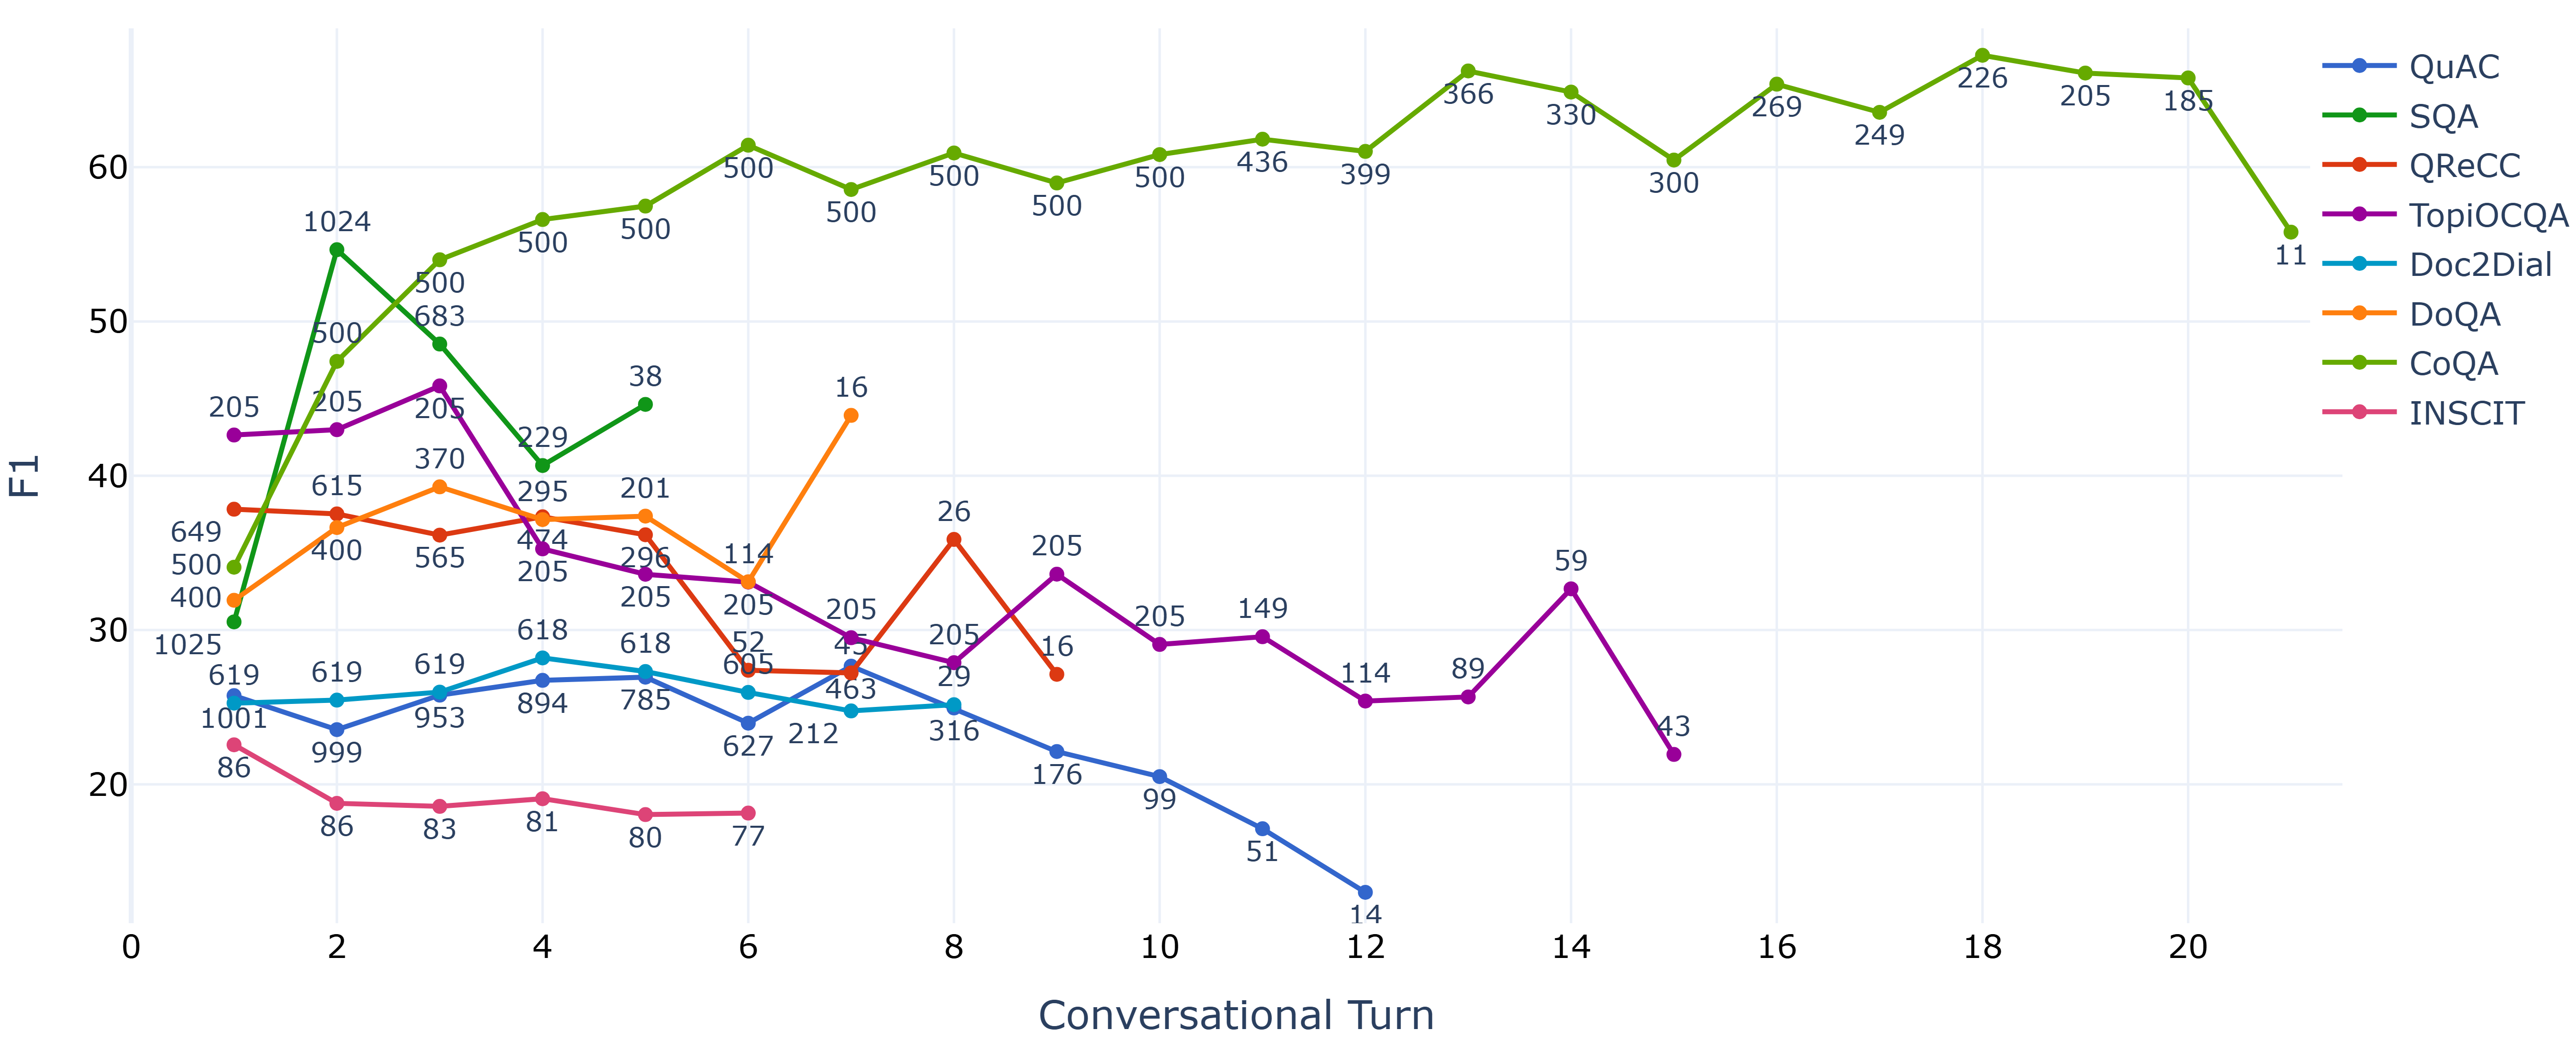
\includegraphics[width=1\linewidth]{plots/conv_f1.png}
  \caption[F1 development over conversation turns]{F1 performance across conversational turn for each dataset using \textit{Vanilla RAG}.}\label{fig:conv_f1_lim}
\end{figure*}

\end{document}
